\chapter{Introduction}
With this chapter, the reader should be able to comprehend why this thesis was written, 
what it tries to accomplish and which topics are considered within the scope of this work.

\section{Motivation}

The increasing amount of Platform-as-a-Service (PaaS) solutions, cloud-hosted environments, containerized workloads and microservice architectures introduce new attack scenarios. 
This creates the need for new defense strategies in both Development and Operations. 
Especially solutions providing Kubernetes (k8s) compliant container orchestration are identifiably different and in high demand compared to long established solutions. 
This calls for a more detailed, focused examination. 

\section{Objective} \label{goal}

This thesis aims to answer the following questions:

\begin{itemize}

\item What generic security risks emerge when providing or using a multi-tenant PaaS solution,
with each tenant developing, deploying and running their own applications? 

\item How can a PaaS provider (serving internal and/or external users) mitigate those risks? 

\item  In this scope and from a PaaS provider viewpoint, how does an on-premise solution compare
to a public cloud solution? 

\end{itemize}

Another goal is to recommend security measures for different implementation use cases.
A comparison of existing risks and the need for action derived from it should serve as central point of view. 
Possible measures to mitigate those risks shall be explored, evaluated and exemplary put to use in practical examples.
Subsequently the risk will be re-evaluated in order to illustrate a viable risk management method.
With the results gathered, the thesis will compare different best practice implementations for different use cases and recommend measures for each.

\section{Scope limitation} \label{scopeLimit}

The thesis will first limit the view on the problem to a manageable scope by concentrating on the components enabled by default and those required for operations of two established and \gls{k8s} compliant solutions.
These solutions will be \gls{ocp} as an on-premise solution and \gls{aks} as a public cloud solution. 
The latest stable version of \gls{ocp} during the work on this thesis was version 3.11\footcite[][, see headline and date]{ocpRelease}, which is based on v1.11 of \gls{k8s}.
Although \gls{k8s} v1.13 was already available through \gls{aks} at the same point in time (see figure \ref{aksVersionsMay}), the available v1.11 was chosen to improve comparability.

The components of these two solutions providing \gls{k8s} compliance will be the main focus, as these bear the most significance across all Kubernetes Certified solutions. 
A look at popular tools and frameworks used in such clusters will be avoided in order to keep the scope manageable, though some might be recommended as a mitigation.
In order to be applicable to a higher number of use cases, attacks and measures seen in environments with exceptionally high security requirements might be mentioned, but not  covered in their entirety. This includes state-sponsored actors deploying zero-day exploits, which are not applicable to a majority of solutions deployed and thus disregarded for the given context.
This thesis aims to provide insight to the risks of providing a PaaS solution and mitigation thereof. 
As such, it will look at the capabilities a potential provider has to (mis-)configure such solutions - inherent risks of the technologies themselves are only explored when measures to mitigate them are accessible from a provider standpoint. 
In short, the goal is to improve the security of a given \gls{k8s} cluster, not \gls{k8s} itself.
To follow the \gls{owasp} Risk Rating Methodology\footcite{riskRating} down the line, we need to define our threat actors and group them when applicable\footcite[][, Section 'Define all possible threats']{threatModeling}. Examining a list of threat actors published through SANS\footcite[][p. 12 to 17]{sansThreatActors}, we will only exclude state-sponsored actors. This leaves us with cyber criminals, hacktivists, systems administrators, end users, executives and partners.
Grouping the remaining actors by the factors used to estimate risks in section \ref{riskEstimate}, we can identify find three scenarios that encompass all of the actors:
%TODO Mention baseline security in summary!
%TODO change summary to fit the items here!
\begin{itemize}

\item Malicious third party attacking the solution from within the company network and/or the internet

\item Malicious third party attacking from inside a hijacked container, i.e. remotely executing code or commands

\item Bad user, i.e. a negligent, hijacked or malicious account risking compromise of their own and/or other applications

\end{itemize}

\section{Research basis and its limits}

During the research for this thesis, a considerable amount of sources has been examined. Surprisingly, very little has been found regarding a risk-based point of view on \gls{k8s} solutions. A lot of sources start with measures and end with attacks, including one of the few published books\footcite{k8sBook}. They recommend specific security measures an explain the sort or attacks they defend against. The only commonly referenced source that specifically introduces major risks for container technologies, without rating them, is the NIST Application Container Security Guide.\footcite{nistK8s}
In addition to that, many of them are still work in progress or outdated.

Some of the sources commonly referenced include (in alphabetical order):
\begin{itemize}

\item The \gls{cis} Docker Benchmark\footcite{cisDocker}

\item The \gls{cis} Kubernetes Benchmark\footcite{cisK8s}

\item The book "Kubernetes Security - How to Build and Operate Applications Securely in Kubernetes"\footcite{k8sBook}

\item The NIST Application Container Security Guide\footcite{nistK8s}

\item The \gls{owasp} \gls{csvs}\footcite{csvsGithub}

\item The \gls{owasp} Docker Top 10\footcite{dockerTop10Github}

\end{itemize}

Other sources include solution specific advisories, i.e. for \gls{k8s} in general\footcite{k8sDocsSecurity} as well as \gls{ocp}\footcite{ocpSecTips} and \gls{aks}\footcite{aksSecTips} specifically. In addition to that, recorded and openly available talks by different people in the industry are available. Especially the talks at KubeCon, the annual \gls{k8s} conference, are accessible through the \gls{cncf} YouTube presence\footnote{Channel Link: https://www.youtube.com/channel/UCvqbFHwN-nwalWPjPUKpvTA/videos}. The speakers include recognized people in the industry, contributors to the \gls{k8s} project and employees of reputable companies like Google, Red Hat and Microsoft.
A considerable number of other online sources were referenced in the sources above or found with online search engines.
These common recommendations exist, but neither claim to be exhaustive nor applicable to all future versions. In case of the \gls{cis} benchmarks, they are not even intended to be followed in full, but just as basis for security considerations.\footcite[][, starting at 29:18]{cisJustRecommendation}
In accordance to this, the findings can only be provided on a best-effort basis and not without reservation towards possible changes through future software versions or new information. This should be an information basis and approach for rating your own implementation while taking the business risk into consideration, not a definitive guide to all aspects in this regard.
As with all systems, new attacks and vulnerabilities may emerge at any point in time. With sufficient research, the chance to have identified the most common attack vectors is probable but the limitations of this research has to be emphasized.

%TODO full list of sources in appendix & reference here?

\chapter{Theory}
With this chapter, a reader with foundational knowledge of topics regarding Computer Science and/or Informatics 
will be able to grasp the specialized technologies discussed within the thesis and familiarize themselves with the definitions and terminology used throughout it.

\section{Infrastructure-as-a-Service}
In \gls{iaas} environments, a consumer delegates the management and control of the infrastructure needed to deploy his applications to his \gls{iaas} provider.
The provided service ends at provisioning of processing, storage, networks and other computing resources.\footcite[][p. 2 to 3]{nistcloud}
Therefore consumers do not need to manage their own data centers or topics like system  availability.
As shown in Figure ~\ref{fig:servicecomparison}, consumers are responsible for the OS layer and everything above it.

\begin{figure}[H]
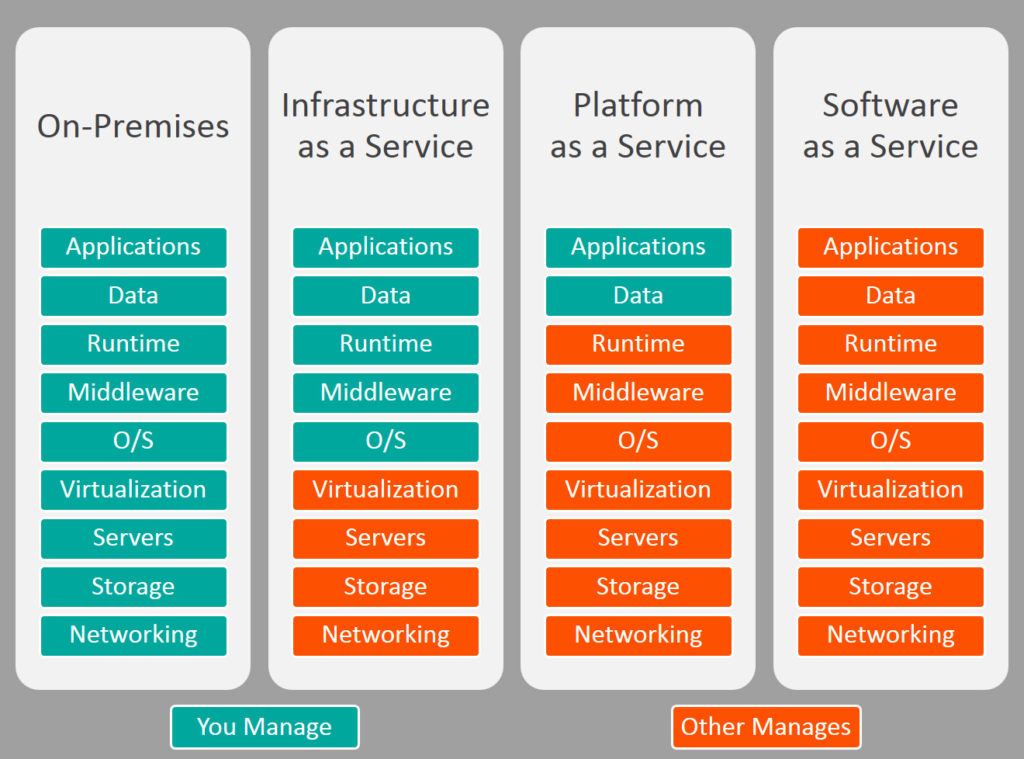
\includegraphics[scale=0.4]{pictures/ServiceComparison.jpg} 
\caption{Comparison of responsibilities in different service models\protect\footcite[][, section 'Original reference image']{servicecomparison}}
\label{fig:servicecomparison}
\end{figure}

\section{Platform-as-a-Service}

In \gls{paas} environments, a consumer delegates the management and control of even more resources needed to deploy his applications to his \gls{paas} provider, beyond those covered by \gls{iaas}.\footcite[][p. 2 to 3]{nistcloud}
In an ideal scenario, this leads to a consumer not having to concern himself with the underlying network, hardware, servers, operating systems, storage or even common middleware like database management or log collection and analysis\footcite[][, section 'Advantages of PaaS']{msPaas} and allows him to focus on other tasks, i.e. application development.
As a downside to this, a consumer might only have limited control on, among other factors, the software installed on the provisioned machines. 
Although this shifts some of the responsibility burden towards the provider, the situation isn't as clear-cut as one might think. 
Figure ~\ref{fig:servicecomparison} shows middleware and runtime as provided, but there is no clear standard on what capabilities or tools are included.
A consumer might require capabilities which aren't provided or wishes to avoid provider lock-in through proprietary tools, 
resulting in some middleware responsibilities falling back to the consumer. 
A consumer might also have to extensively configure or modify the application-hosting environment for compliance or security purposes. 
Even some low-level tasks aren't completely managed, i.e. \gls{vm} reboots to apply security updates.\footcite[][, section 'Process Linux node updates and reboots using kured']{msVmReboot}

\section{Containers}

Unsurprisingly, a basic building block of running containerized applications are containers.
In order to run and manage containers, several components and systems are needed. The most important ones will be introduced here.

\subsection{What are containers?}
A container is a standard unit of software that packages up code and all its dependencies so the application runs quickly and reliably from one computing environment to another.\footcite[][, section 'Package Software into Standardized Units for Development, Shipment and Deployment']{whatContainer}
From a technical viewpoint, a container is an isolated process running in the userspace of a host OS. The host system shares the kernel with all containers on it and might share other resources, but containers are run from container images which include any code and dependencies needed in order to make them independent of the infrastructure they are running on (except the kernel).\footcite[][, slide 13]{containerIntro}

Linux containers were widely popularized through Docker, a container system initially based on \gls{lxc}.\footcite[][, section '2013: Docker']{containerHistory}
Containers provide isolation of multiple applications running on the same machine and are often deployed in environments where this isolation would formerly have been achieved by using multiple \gls{vm}s. Thus, they are often compared to them despite the fundamental technical differences. The Kubernetes documentation illustrates the differences as seen in Figure ~\ref{fig:VMsVsContainers}.

\begin{figure}[H]
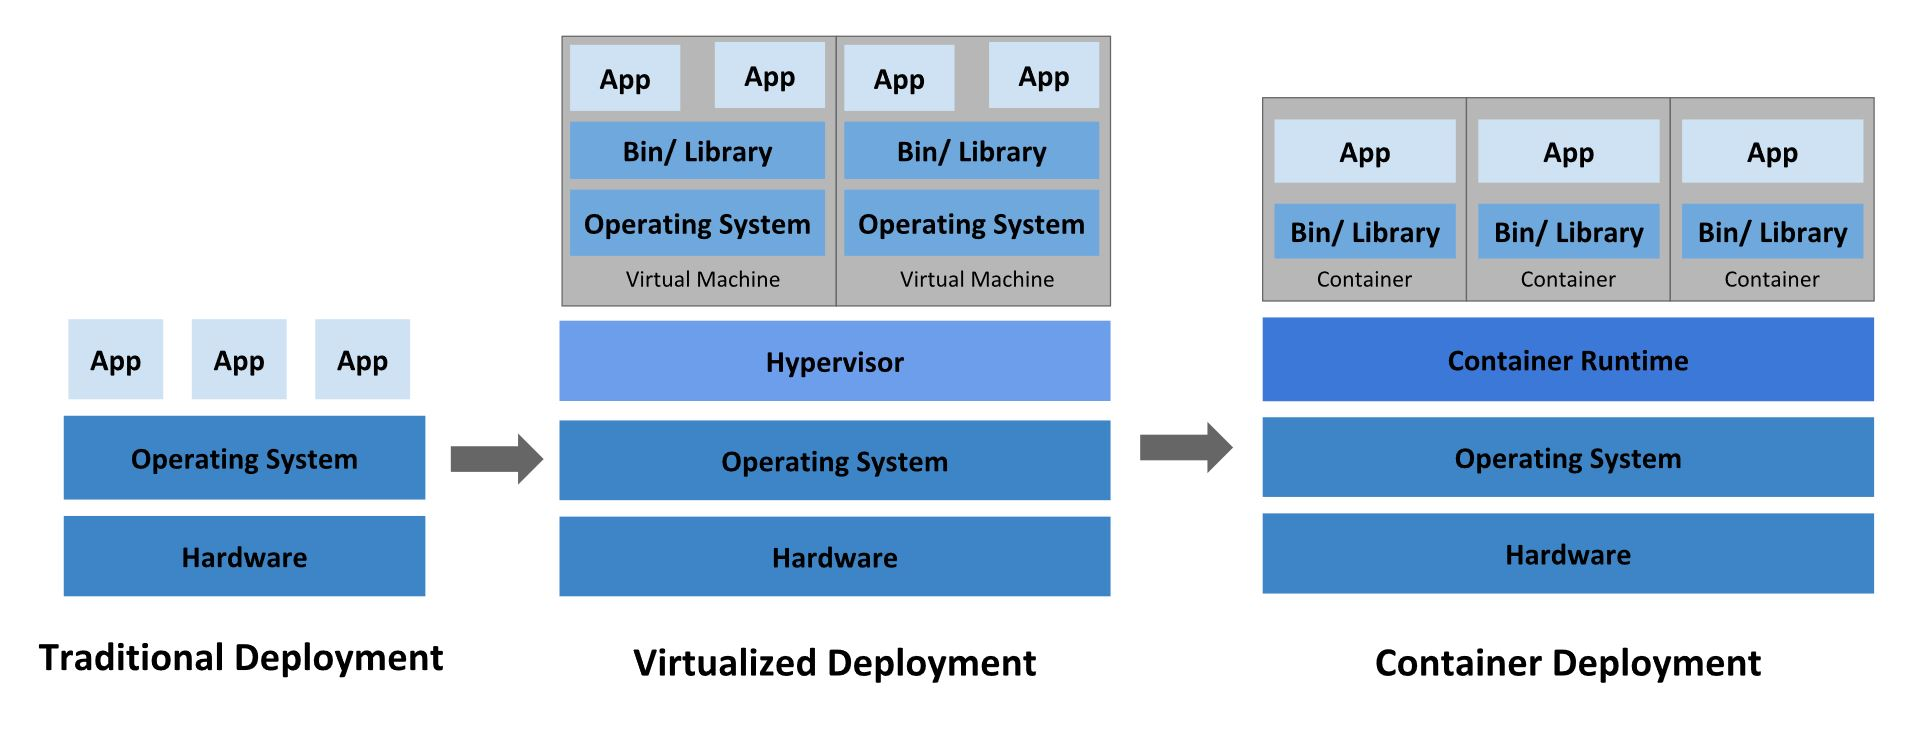
\includegraphics[scale=0.3]{pictures/VMsVsContainers.jpg} 
\caption{Comparison of different application deployments on the same hardware\protect\footcite[][, section 'Going back in time']{k8sBasics}}
\label{fig:VMsVsContainers}
\end{figure}

\subsection{Differentiating docker}
Talking about docker can be quite difficult, since the term is overloaded with different meanings - a company (Docker Inc.), their commercial products (Docker CE and Docker EE) and the former name of their open source project (formerly known as Docker, now called Moby).\footcite[][, section 'What is Moby?']{dockerMoby}
Additionally, there is a \gls{cli} called docker engine, which serves as an interface to the containers running on a host. It includes a high-level container runtime\footcite[][, section 'Develop, Ship and Run Any Application, Anywhere']{dockerEngine}, which will be talked about in the section \ref{runtimes}.
Some sources also talk about docker-formatted containers when those technologies implement the same interfaces as the docker container runtime.\footcite[][, section '1.11. Working with Docker formatted containers']{dockerFormatted}

\subsection{Images, image building and Dockerfiles}
A container image is a binary including all the data needed to run a container. It might also contain metadata on its needs and capabilities, i.e. version information through tags.\footcite[][, section 'Docker Images']{redhatImages}
Container images are sometimes referred to as docker images or docker-formatted images, but they can be run by other container runtimes and vice versa.
In order to create a container image, you have to build it. This is often done through a build process executed by a container runtime. The instructions for container builds are commonly defined and documented in a Dockerfile\footcite[][, section 'Dockerfile reference']{dockerfileDocs} (which may also be done by non-docker programs, adding onto the vocabulary confusion).
Container images can be distributed through container image registries, where images can be uploaded to and downloaded from. A commonly known example is docker hub, a public registry run by Docker Inc.

\subsection{Container standards and interfaces} \label{runtimes}

Without going into the nuances and historical developments, there are a multitude of programs mostly implementing three interfaces for container management.
The two basic interfaces are the runtime and image specifications under the \gls{oci} which standardize how containers and container images should be formatted and executed.\footcite[][, first paragraph]{ociStandards}
The \gls{oci} also maintains a commonly used reference implementation called runc, alternatives include rkt and lmctfy.\footcite[][, section 'Examples of Low-Level Container Runtimes']{lowLevelRuntimes}
Runc and similar programs implementing these specifications are commonly called low level runtimes, in contrast to the high level runtimes that control them.
These high level runtimes like containerd or CRI-O commonly manage more abstract features like downloading and verifying container images.\footcite[][, Intro and section 'Examples of High-Level Runtimes']{highLevelRuntimes}
Many high level runtimes today adhere to the \gls{cri} so they can be used interchangeably by container orchestrators.\footcite[][, section 'Purpose']{criGithub}

%TODO maybe shorten and just talk about CRI upwards?

\section{Container orchestration}
Once you want to use multiple containers on different machines talking to each other and offering stable services that continue even when a container or machine fails, the need for automated systems to manage these containers arises. Orchestrators can also provide other advantages like load balancing and automated scaling.
Kubernetes systems are popular orchestrators currently in use.
The sum of hosts running the orchestrator and containers are called a cluster.
%TODO citation for kubernetes market share?

\subsection{Kubernetes} \label{k8sTheory}
At its core, \gls{k8s} is a control system for containers.
It constantly compares the current state with the set target state and tries to correct towards the target when needed, i.e. when a container crashes.
The intended way for a user to deploy or change their application is to adjust the target state and let the \gls{k8s} system take care of the rest.\footcite[][, section 'Understanding Kubernetes Objects']{k8sObjects}
There are many \gls{k8s} distributions, many of which are certified Kubernetes offerings, meaning they all comply to the same standards and interfaces. These are set by the Linux Foundation through the \gls{cncf} which oversees the project.
The Kubernetes code base is open source and maintained on GitHub, but any implementation fulfilling the (publicized) requirements can become \gls{k8s} certified, regardless of how much code they changed.\footcite[][, section 'There are over 80 Certified Kubernetes offerings.']{certifiedK8s} You could look at \gls{k8s} as a standardized interface for container orchestration with a public reference implementation.

\subsubsection{Kubernetes components} \label{k8sComponents}

In order to deliver a working \gls{k8s} cluster, multiple (binary) components are needed.
Master components provide the control plane, while node components are run on each underlying machine in order to maintain and provide the environment to execute the containers you want to run eventually.
Master components are often exclusively run on machines dedicated to them, which are called master nodes - in contrast to worker nodes, which run the containers your applications consist of.\footcite[][, section 'Master Components']{k8sComponents}

The most relevant master components from the perspective of this thesis are:
\begin{itemize}

\item The kube-apiserver, which exposes the Kubernetes API. It is the front-end for the Kubernetes control plane; Cluster user or Administrator commands are typically directed at and processed by this component.

\item Etcd, a distributed high-availability key value store where, among other things, secrets and authentication information are stored.

\end{itemize}

The important node components include:
\begin{itemize}

\item The kubelet, an agent running on each node in the cluster. It mostly monitors the state of any containers started by the \gls{k8s} cluster. These are run through pods, a Kubernetes object designated to executing containers. The kubelet also interacts with the master components and reports on the monitoring data.

\item The container runtime as depicted in figure \ref{fig:VMsVsContainers}, which is responsible for actually running containers. Examples include \gls{ocp} using Docker while \gls{aks} uses Moby, but any implementation of the \gls{cri} is supported.\footnote{For additional information, refer to section \ref{runtimes}} 

\end{itemize}

Figure \ref{fig:k8s-big-picture} illustrates these components in context. It is to note that users in this illustration are the users of the applications running in the cluster; From a provider standpoint the users would be the people responsible for development and operations.

\begin{figure}[H]
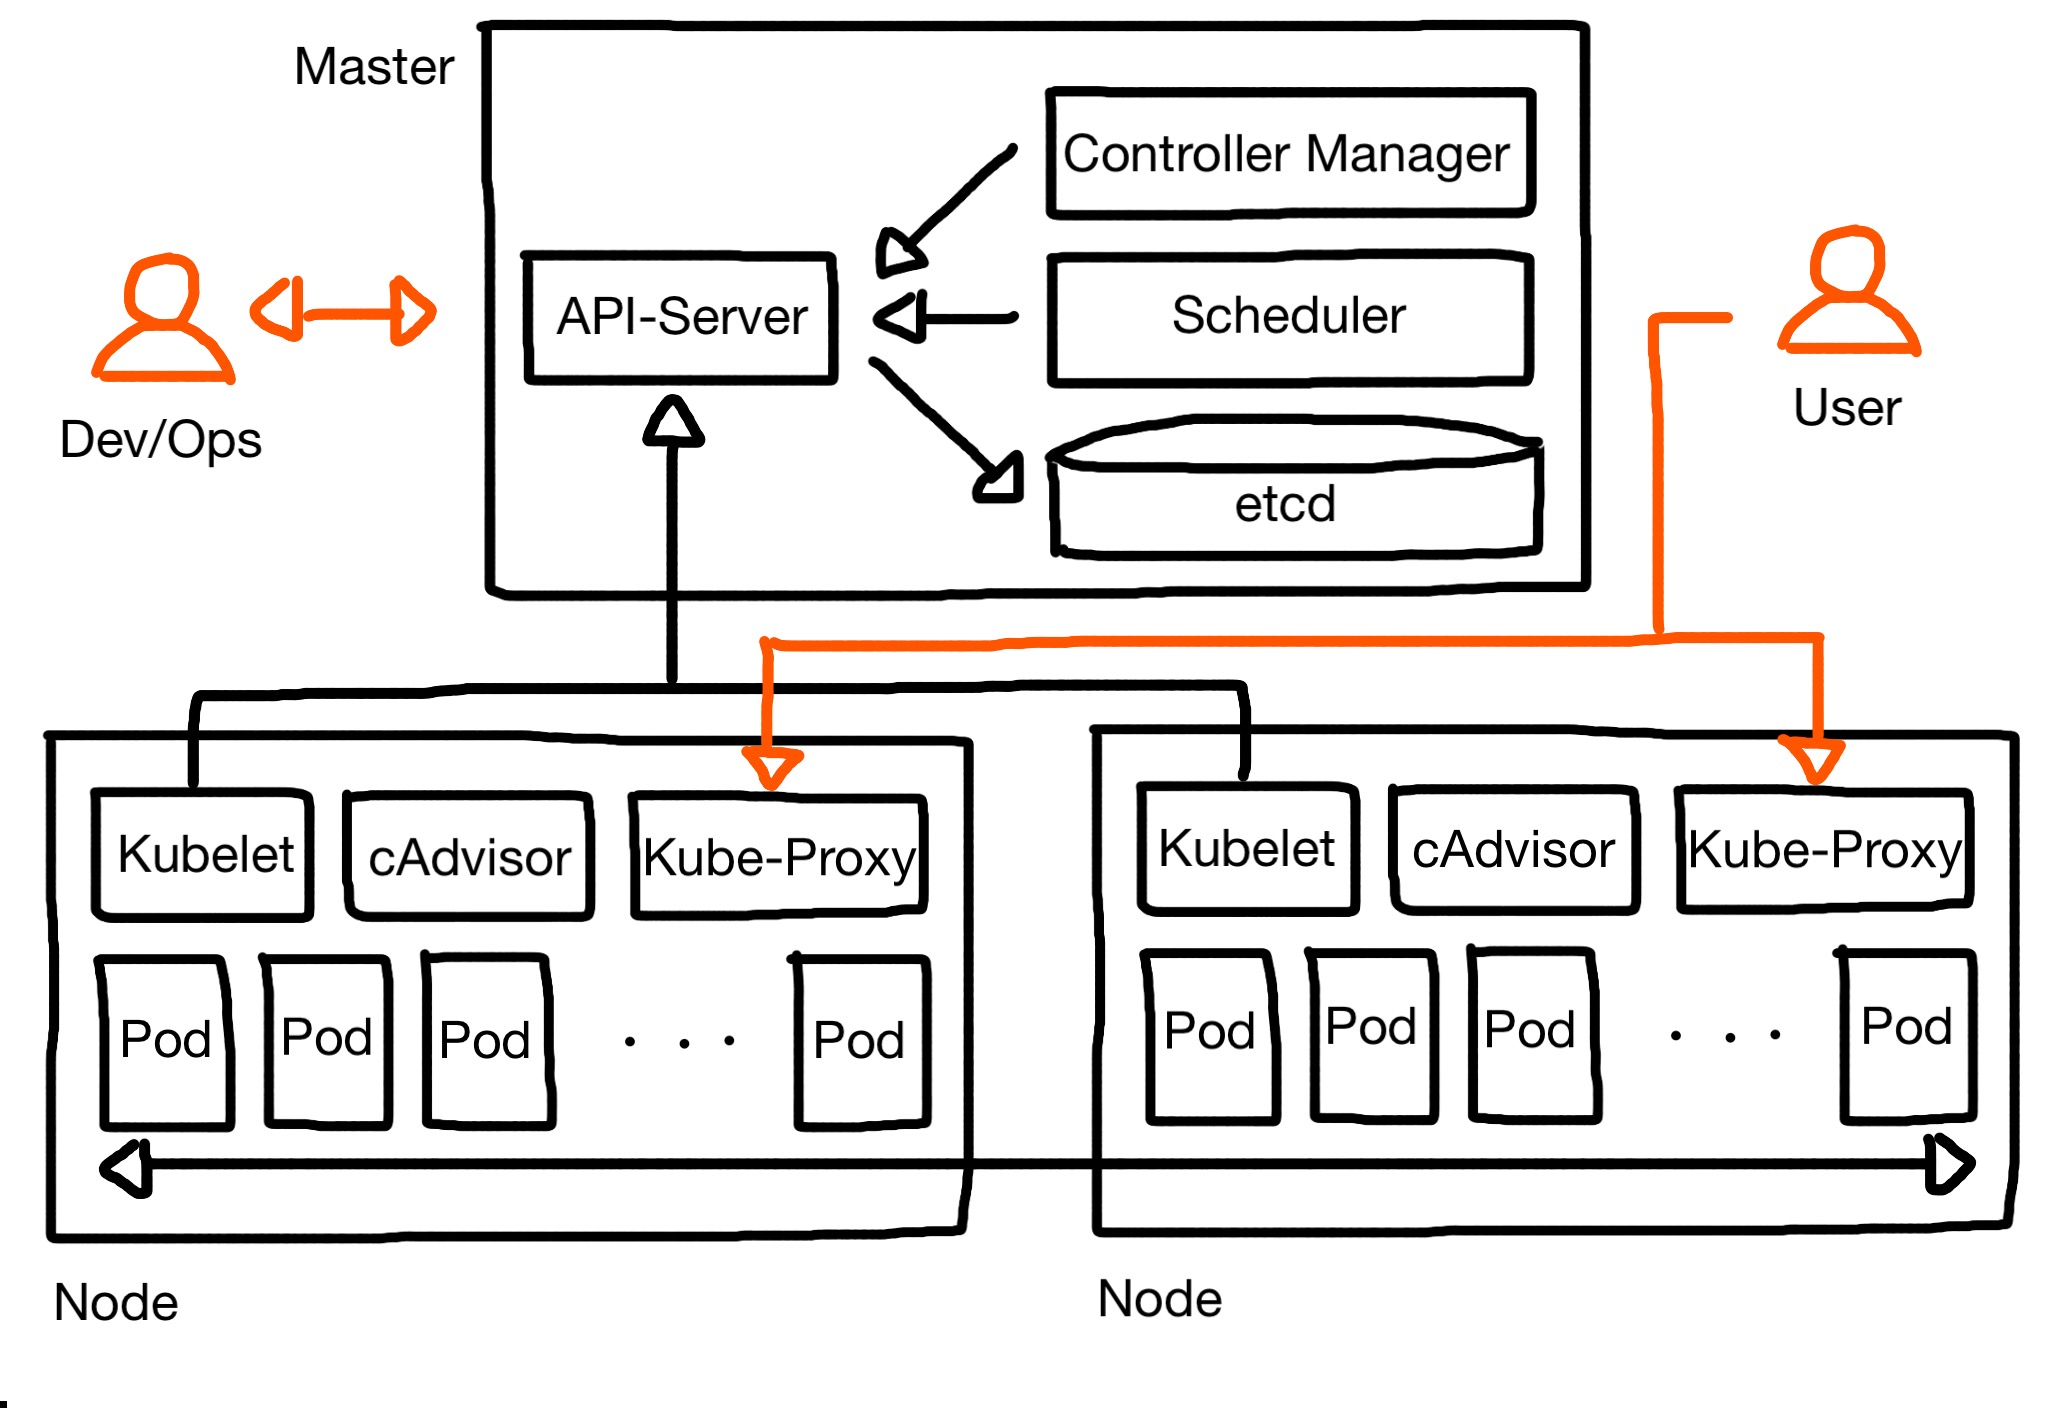
\includegraphics[scale=0.2]{pictures/big-picture.JPG} 
\caption{An overview of different \gls{k8s} components\protect\footcite{nicoPictures}}
\label{fig:k8s-big-picture}
\end{figure}

%TODO component functions and number may vary per distribution

\subsubsection{Kubernetes objects}
Kubernetes objects are persistent entities that represent the desired state of your cluster. They can describe what containers should run, which resources are available to what system and the policies to apply (i.e. automatic restart behavior and communication restrictions).
The intent is to modify these objects in order to change the target state, which the \gls{k8s} system then works towards by adjusting the current state to match.\footcite[][, section 'Understanding Kubernetes Objects']{k8sObjects}
Some objects, i.e. pods, belong to a specific namespace, meaning a virtual cluster of many in a shared physical cluster. Others, like node objects describing the underlying machine, exist outside of a specific namespace.
In order to understand how one can make the \gls{k8s} system run an application according to its requirements, an understanding of the basic objects is needed.
%TODO make object names bold/italics? also do that to all other important names/definitions in the theory chapter?

A pod is the basic \gls{k8s} object and encapsulates a container with some resources like an IP, storage and policies. Pods are typically each comprised of one container, a single instance of an application in \gls{k8s}. They may contain more than one container for cases where these are tightly coupled and directly share resources.\footcite[][, section 'Understanding Pods']{k8sPods}
That's all the pods do. They run.\footcite[][p. 4]{phippy}

Pods are usually not created manually, but started and stopped by a replicaSet. Their purpos as a \gls{k8s} controller is to maintain a stable set of replica pods running at any time in order to ensure availability of the function this type of pod provides.\footcite[][, introductory sentence]{k8sReplicaSets}

ReplicaSets are in turn managed by deployments. Just as replicaSets control pods, deployments control replicaSets in order to maintain the currently desired state of a cluster.
Figure \ref{fig:k8s-deployments} illustrates this connection.

\begin{figure}
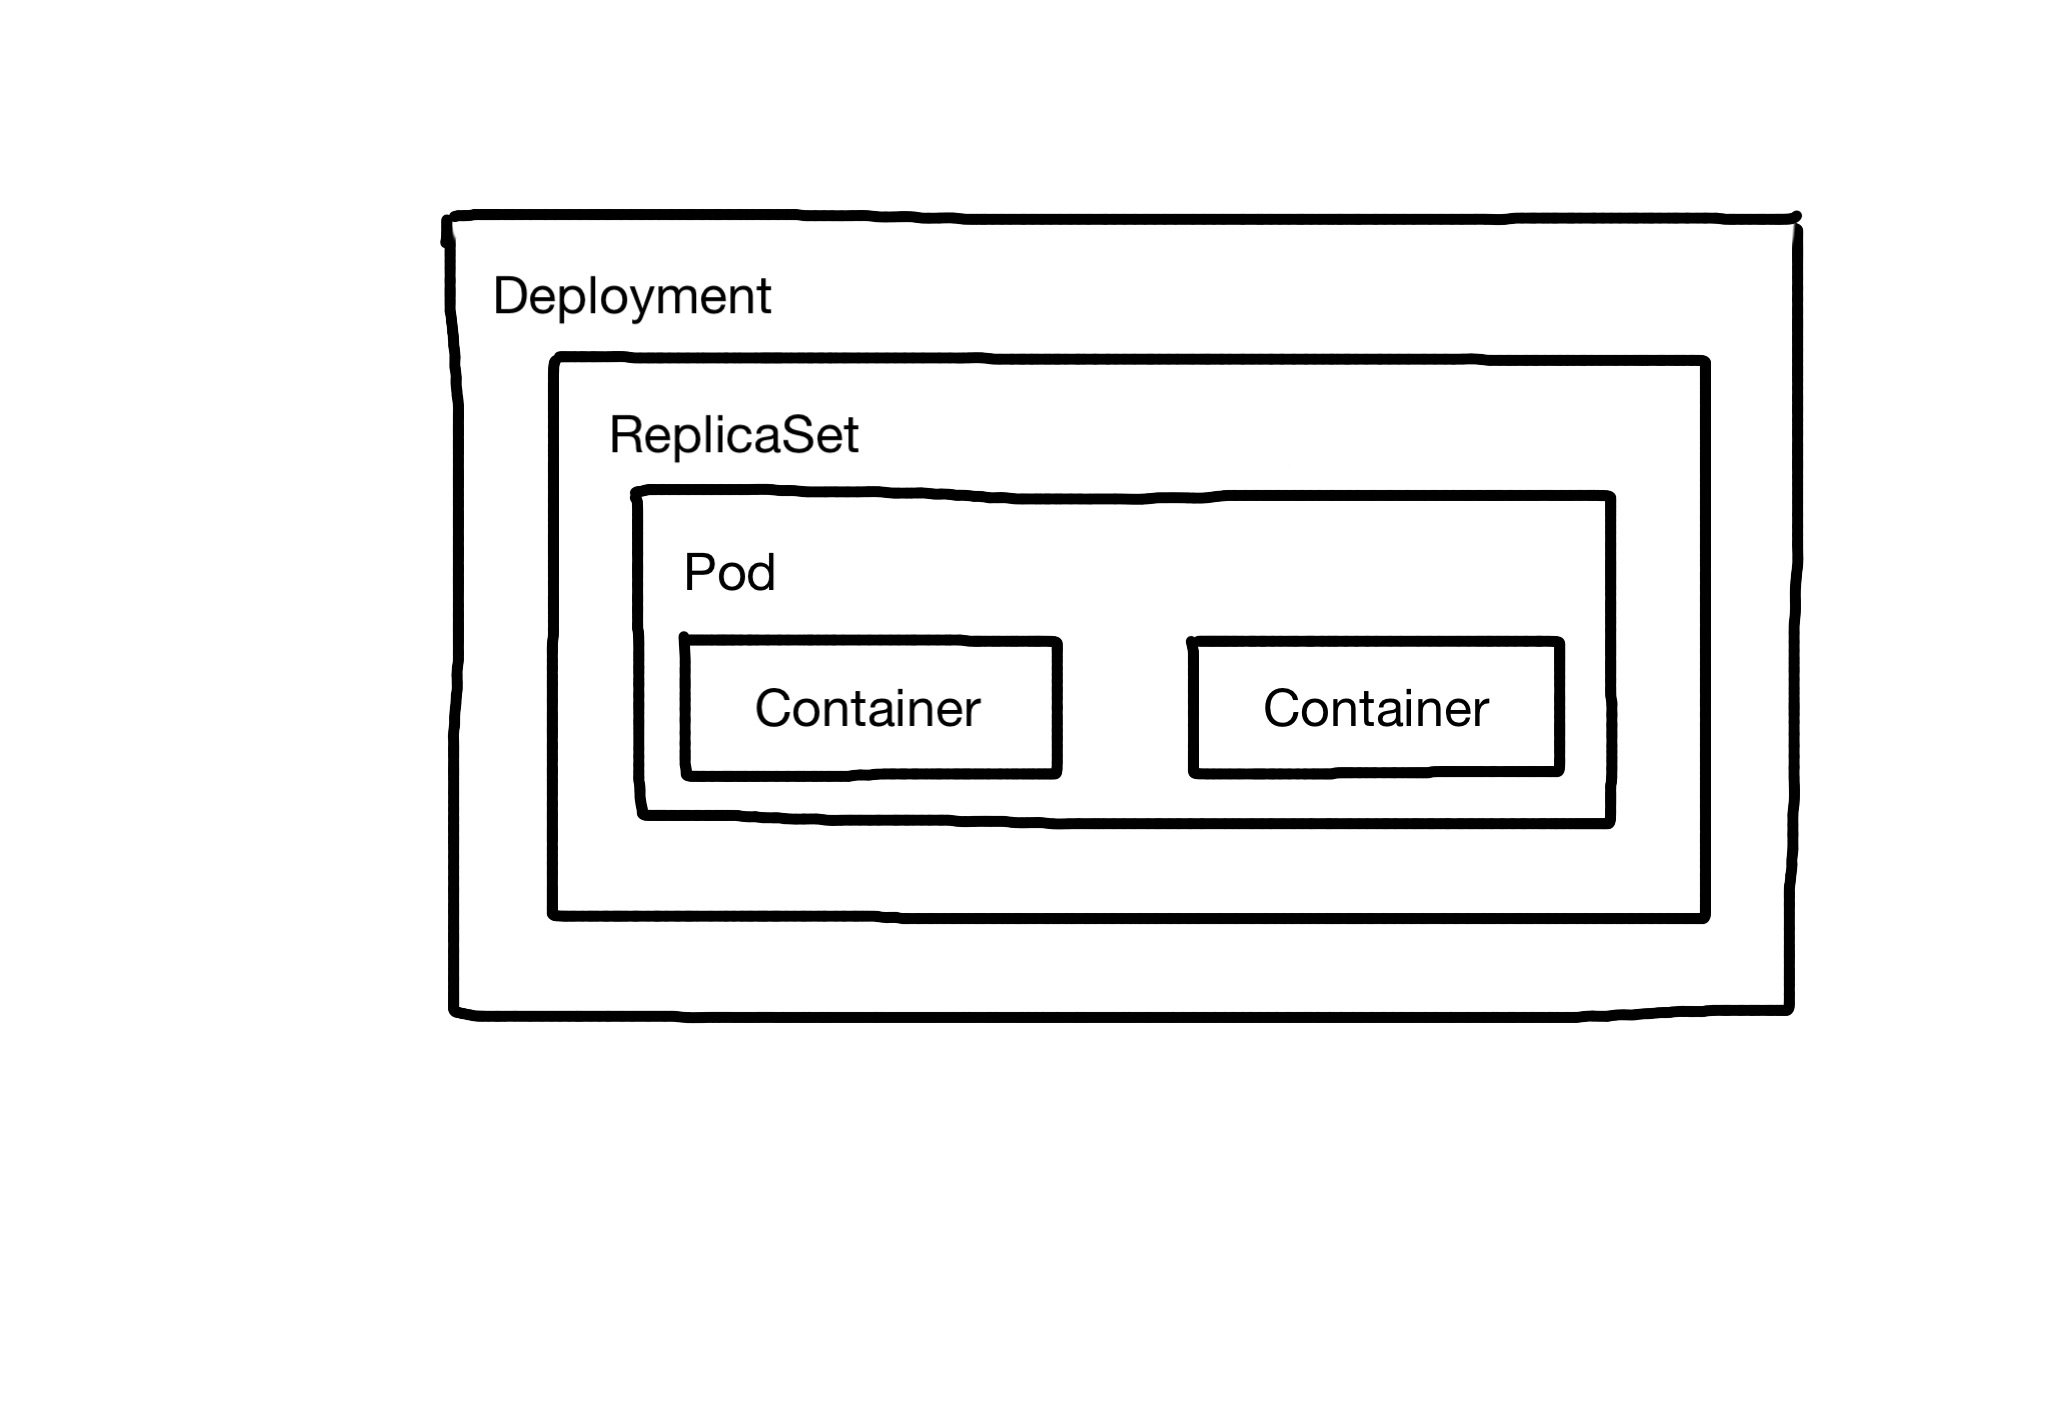
\includegraphics[scale=0.2]{pictures/deployment.JPG} 
\caption{Connection between deployments and other \gls{k8s} objects down to containers\protect\footcite{nicoPictures}}
\label{fig:k8s-deployments}
\end{figure}

Since multiple identical pods may provide the same functionality and instances of this type of pod could be stopped or started at any point, how could a pod or other system address and connect to a pod? This can be solved by configuring a service, which abstracts a set of pods and their access policy. Typically, you talk to services instead of other pods directly. These services might then be published cluster-externally, i.e. through a load balancer provided by a cloud provider as seen in figure \ref{fig:loadbalancer}.

\begin{figure}
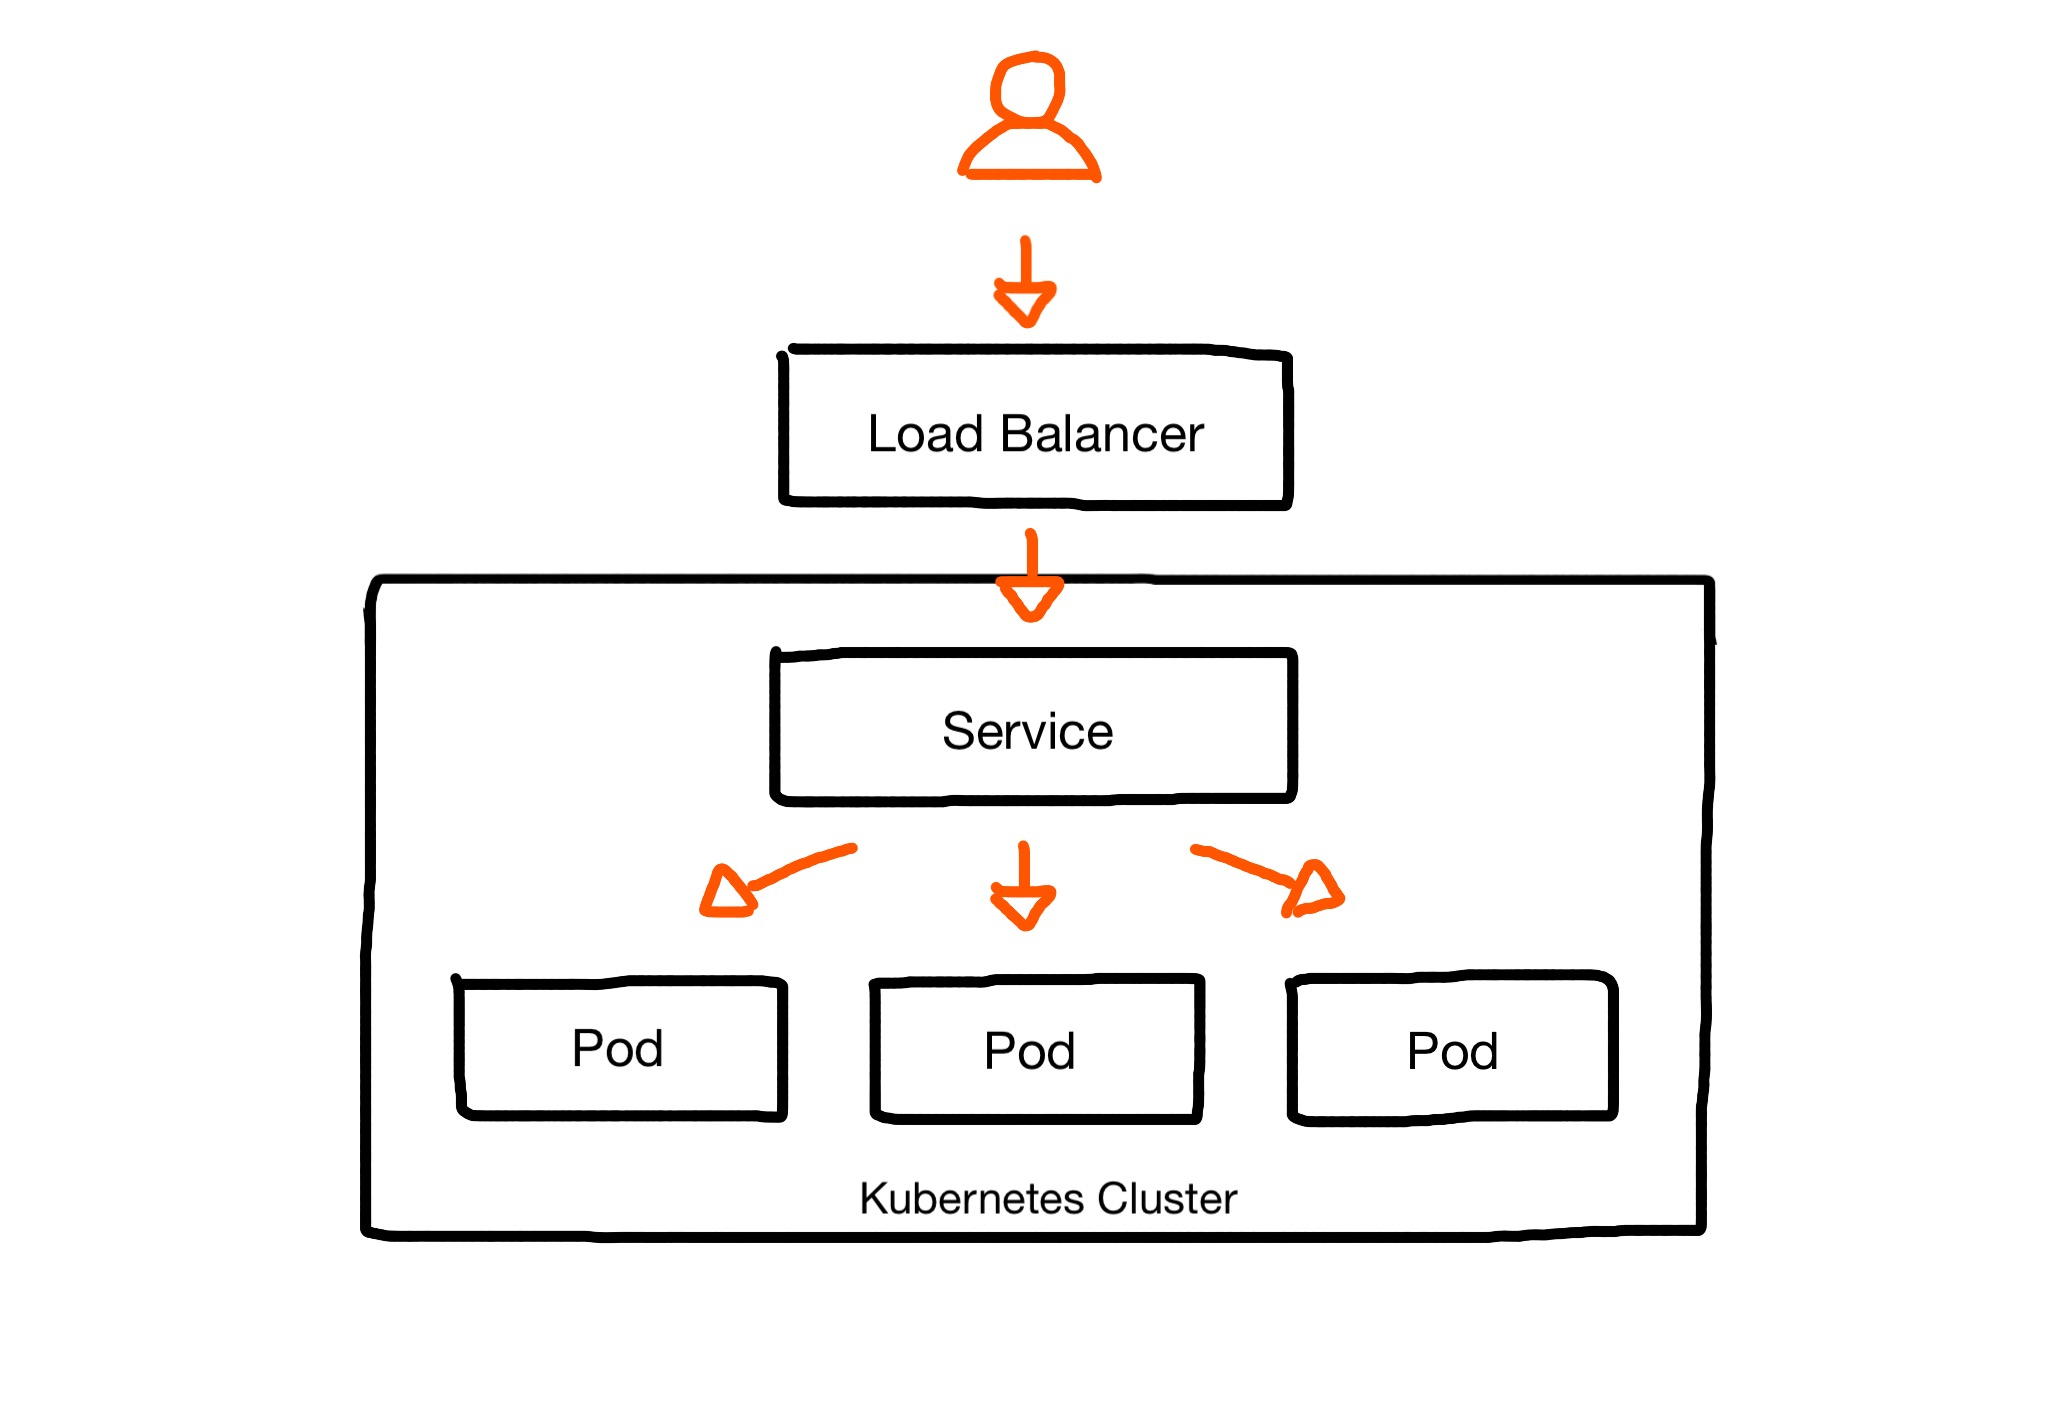
\includegraphics[scale=0.2]{pictures/loadbalancer.JPG} 
\caption{Connection between deployments and other \gls{k8s} objects down to containers\protect\footcite{nicoPictures}}
\label{fig:loadbalancer}
\end{figure}

%TODO other objects: volumes, daemonsets, podsecuritypolicies, networkpolicies, (others needed/referenced?)

\subsubsection{Using Kubernetes}
There are many ways and solutions to set up a \gls{k8s} cluster. Anyone can write their own one from scratch, but so-called turnkey solutions for cloud and on-premise environments exist, too, which significantly reduce the time and effort required to set up and run a cluster.\footcite[][, sections 'Turnkey Cloud Solutions' and 'On-Premises turnkey cloud solutions']{turnkey}
%TODO maybe: buy CaaS/PaaS/IaaS, cloud vs. on-prem, different scopes/features from different products
Once your cluster is set up, it is typically interacted with through the \gls{k8s} API. For human interaction, kubectl is a \gls{cli} reference implementation which enables remote interaction with it.\footcite[][, section 'The Kubernetes API']{k8sApi}
In order to create or manipulate an object, you need to provide its new specification. This is typically supplied to kubectl as a .yaml file, an example of which can be seen in listing \ref{lst:example-yaml-file}.\footcite[][, section 'Describing a Kubernetes Object']{k8sObjects}

\begin{lstlisting}[
	caption={Exemplary .yaml file of a simple k8s deployment\protect\footcite{k8sObjects}},
	label={lst:example-yaml-file}]
apiVersion: apps/v1 # for versions before 1.9.0 use apps/v1beta2
kind: Deployment
metadata:
  name: nginx-deployment
spec:
  selector:
    matchLabels:
      app: nginx
  replicas: 2 # tells deployment to run 2 pods matching the template
  template:
    metadata:
      labels:
        app: nginx
    spec:
      containers:
      - name: nginx
        image: nginx:1.7.9
        ports:
        - containerPort: 80
\end{lstlisting}

%TODO custom yaml highlighting? https://tex.stackexchange.com/questions/152829/how-can-i-highlight-yaml-code-in-a-pretty-way-with-listings/152856#152856

\subsection{OpenShift} \label{openshiftExplanation}

OpenShift is a commercial Kubernetes container platform by Red Hat. There are several different options to choose, deployable in different environments. OpenShift Online is hosted in a public cloud, while OpenShift Dedicated is hosted on dedicated nodes in a virtual private cloud. The option most relevant to this thesis is \gls{ocp}, which can be deployed on any infrastructure, including on-premise environments.\footcite[][, section 'OpenShift plans and pricing']{openShiftOptions}
Red Hat sponsors and supports the development of Fedora, a Linux distribution on which they base their \gls{rhel} OS on. \gls{rhel} is then used by them commercially by supplying its binaries and updates through commercial licenses.
Similar to this, Red Hat develops and supports a \gls{k8s} distribution called \gls{okd}, which then serves as a base for their OpenShift products, including \gls{ocp}.\footcite[][, section 'OKD vs Red Hat OpenShift']{ocpVsOkd}
\gls{okd} release versions correspond to the \gls{k8s} version it is based on, i.e. \gls{okd} 1.11 is based on \gls{k8s} 1.11.\footcite[][, section 'What is OKD?']{okd}
\gls{ocp} versions may differ, but Red Hat maintains a list of tested integrations for each major \gls{ocp} release, giving insight to which \gls{k8s} version it is based on.\footcite[][, table 'Platform Components']{ocpK8sVersions}
\gls{ocp} is a certified Kubernetes distribution, which means it implements the same interfaces as all the others.\footcite[][, table 'Platform - Certified Kubernetes - Distribution']{certifiedK8s}
Despite this, the differences in intended usage become apparent quite quickly, starting with the \gls{cli} used to interact with a cluster (oc instead of kubectl).\footcite[][, section 'Basic Setup and Login']{ocpCli}
Even basic concepts like namespaces are different, as \gls{ocp} uses the similar but not identical concept of projects.\footcite[][, section 'Overview']{ocpProjects}
\gls{ocp} uses Docker as its container runtime by default, but CRI-O is another option.\footcite[][, section 'Getting CRI-O']{ocpCrio}

\subsection{Azure Kubernetes Service}

The Azure Kubernetes Service is a managed \gls{k8s} solution offered by Microsoft and running in the Azure public cloud. 
As it does not differ from the \gls{k8s} reference implementation compared to \gls{ocp}, its functionality is identical to the general \gls{k8s} mechanics described in section \ref{k8sTheory}.
The computing resources used to run the cluster are pre-configured and provisioned \gls{vm}s in the Azure cloud, which do not need to be configured and run a container runtime based on Moby, a toolkit from which the Docker runtime is built.\footcite[][, section 'What is Moby?']{dockerMoby} 
\gls{k8s} versions in \gls{aks} directly correspond to the \gls{k8s} version they are based on.
As many cloud services do, there are multiple integrations to other cloud services, in case of \gls{aks} including an option to integrate your Azure Active Directory to authenticate users.\footcite[][, first paragraph]{aadAksAuth}

%TODO any context missing here?

\chapter{Deriving the attack surface and security measures}
%derive all vectors from the three scenarios, explain why you cannot prove that this is/will be everything, explain why grouped this way \& which systems/threat actors rolled together in it. List security measures for each.
%TODO review when done - missed anything of ^this?

Picking up the three scenarios of section \ref{scopeLimit}, we identify the possible attack vectors in this chapter to get an overview of the attack surface that is posed by \gls{k8s} systems. Vectors and the possible attacks by different threat actors are explained as well as possible security measures introduced.

\section{Defining procedure and approach}

The identification of attack vectors within scope turned out to be a big challenge, both in research and preparation for a clear presentation. 
As new minor versions of \gls{k8s} are released approximately every tree months and the Kubernetes project only maintains release branches for the most recent three minor releases\footcite[][, section 'Supported versions']{k8sSupport}, the underlying system evolves continuously. Due to lengthy review processes, accredited literature about the topic are rare and risk being outdated quite quickly. Even less formal sources like blog posts or guidelines published by organizations are both rare, still unfinished at the point of this writing or updated continually, further complicating the creation of a snapshot regarding the current state. Nonetheless, we tried to achieve it on a best-effort basis.
These vectors are applicable to all \gls{k8s} solutions, although the available security measures will vary between different products or implementations. Thus, we will generically mention the applicable measures and may provide specific examples for \gls{aks} and \gls{ocp} for further illustration.
%TODO ^leave 'specific examples in? did you provide any?
In order to give a more comprehensible picture, the scope of these vectors varies. Some areas of interest, i.e. unpatched software and vulnerabilities in the underlying server  infrastructure, have a broad scope. Since they are well known security topics applicable almost all systems, we felt comfortable to broadly encapsulate them for a more clear understanding. If we were to rigorously differentiate between only slightly different vectors, this list would be multiple times as long as it already is.

%TODO say that this is not perfect, but more would be out of scope / no time left?

\section{Identified vectors and security measures} \label{vectorIdentify}
%TODO write out pretty, absorb explanations from risk estimate chapter
The following headlines will each respectively define and explain one of the 17 identified attack vectors of this thesis. For brevity of reference, each has a Vector ID assigned which is formatted as V\textit{xx}.

%TODO
%TODO mention these generic measures
%LOG ALL THE THINGS
%	ELK/EFK-stack or Splunk with log forwarding/aggregation (container AND nodes), k8s audit logging (k8s)
	
%MONITORING AND ALERTING
%	prometheus, grafana (visualization), neuvector, (sysdig) falco, aqua, twistlock


\subsection{V01 - Reconnaissance through interface components} \label{v01}
An attacker could gather information through the available interfaces in order to prepare further attacks and look for vulnerabilities to exploit.
A \gls{k8s} cluster has many interfaces, some of which are intended to be accessed by users or other non-master-components. These components include the kube-apiserver introduced in section \ref{k8sComponents}, the popular web-based \gls{k8s} user interface called Dashboard\footcite[][, first paragraph]{k8sDashboard} as well as solution-specific interfaces like the \gls{ocp} web console\footcite[][, section 'Overview']{ocpWebConsole} or the Azure Portal for \gls{aks}\footcite[][, section 'Create an AKS cluster']{azurePortal}.
Other interfaces are intended to be accessible from inside a cluster. These may include the components accessible from cluster-external sources, but also APIs for the integration of additional functionality. A common use case for such APIs is the provisioning of additional cloud resources in order to scale up the cluster.
One example of reconnaissance against the kube-apiserver was demonstrated at KubeCon 2019\footcite[][, starting at 8:45]{lizReconDemo}, while an example of leveraging the cloud api can be found in a blog post\footcite{aksApiExploit}.

Following the security principle of limiting the attack surface\footcite[][, p. 4 to 5]{k8sBook}, the measures against this include blocking access to or outright deactivating interfaces. If interfaces are unused, i.e. the \gls{k8s} Dashboard where only \gls{cli} tools are used for cluster interaction, one can easily deactivate the Dashboard and thus reduce the attack surface without further work needed. If an interface is used, but alternatives exist, it may be advisable to evaluate whether a change in workflows or software architectures in order to decommission the interface may provide an overall benefit.
Least privilege, another security principle\footcite[][, p. 3 to 4]{k8sBook}, can be followed by restricting access to used interfaces. Authentication can be required of both humans and automated processes and their access may be restricted to the information and capabilities strictly needed to operate. KubiScan, an open source tool to scan the \gls{rbac} permissions of a \gls{k8s} cluster for permissions considered risky, is publicly available to assess a given cluster. Users might be required to log in through a two factor authentication to hinder access through stolen credentials. Network restrictions can be put in place to restrict the vantage points from which an attacker may gain access.
Following Defense in Depth\footcite[][, p. 3]{k8sBook}, this should not only be done from the outside, but access from inside the cluster, too. As an example, most containers don't need access to \gls{k8s} master components, so these requests can be blocked by \gls{k8s} Egress Network Policies\footcite[][, section 'The NetworkPolicy Resource']{egressNetPol}. The impact of successful attacks could be limited through Alerting and restriction of the attacks 'blast radius'. Logging and alerting processes may be implemented through \gls{k8s} audit policies\footcite[][, section 'Audit Policy']{auditPolicy} for requests that are considered suspicious and do not occur in normal operations, examples of which can be found in online sources\footcite[][, section 'Alerting on the Kubernetes infrastructure']{sysdigMonitoring}. The 'blast radius' may be reduced by isolating different applications or teams trough multiple namespaces and restricting access to non-namespaced resources to cluster administrators, thus isolating an attacker to a single namespace instead of the whole cluster. An even more drastic isolation could be achieved through isolation by cluster, resulting in separate \gls{k8s} master components per isolated entity.

\subsection{V02 - Reading confidentials through interface components}
The components mentioned in section \ref{v01} could also be used by an attacker to gather confidential information, which can be either useful in and of itself or used to gain further access. Extracted private keys, tokens or passwords  may be leveraged to authenticate with additional privileges in order to steal or manipulate container images, adjacent applications, source code and interact with other interfaces.

Despite presenting a more serious damage potential, the measures of section \ref{v01} also apply here since they target the same interfaces.
In addition to that, special attention should be paid to the way secrets are passed into code running under \gls{k8s}. Embedding secret information into container images should be avoided, since those are not only unencrypted and difficult to change, but may be extracted by an attacker reading the Dockerfile or inspecting an image themselves. Supplying them through environment variables is also not recommended, as those might be exposed in unconsidered ways. It is recommended to supply them to containers at runtime through \gls{k8s} secrets or external tools like those integrated into cloud platforms or offered by third-party providers. Popular third-party solutions include HashiCorp Vault and CyberArk Conjur.\footcite[][, chapter 7]{k8sBook}

\subsection{V03 - Configuration manipulation through interface components} \label{v03}
With write access to the components mentioned in section \ref{v01}, an attacker may change configurations of the cluster or its environment, i.e. security controls set in place through the cloud provider platform. Examples include disabling security restrictions, rendering alerting processes dysfunctional by blocking their communication or swapping container images with functional, but compromised alternatives.

As this has a higher potential for damage, special care should be taken. The measures of section \ref{v01} are applicable here, too. Special thought may be put into restricting write permissions to the most privileged user accounts, i.e. cluster or cloud administrators for actions that can influence systems outside of a namespace or cluster.
In order to automatically deny actions, \gls{k8s} Pod Security Policies\footcite[][, section 'What is a Pod Security Policy?']{securityPolicy} may be leveraged. Since these are non-namespaced \gls{k8s} objects themselves, they could be circumvented by anyone with permissions to manipulate non-namespaced objects, i.e. cluster administrators.

\subsection{V04 - Compromise internal master components}
In contrast to the components mentioned in section \ref{v01}, there are others which are only intended to be interacted with by other \gls{k8s} master components. They may also be compromised by an attacker. We will refer to these as internal components.
The most promising target is the etcd key value store introduced in section \ref{k8sComponents}, as through it an attacker may gain any permission they want\footcite[][, chapter 'Running etcd Safely']{k8sBook}.

The available security measures are much more straightforward than those of the interface components, which is why all (ab)use cases have been united in one vector.
Master components can be run on any machine in the cluster, but are often run on dedicated master nodes.\footcite[][, section 'Master Components']{k8sComponents}
Therefore, \gls{k8s} solutions can restrict access to these by either not exposing them to anyone outside the pool of master nodes or, in case the components themselves are deployed as containers, restricting write access to their namespace they are running in as well as communication to the containers themselves.
Synonymous to section \ref{v01}, isolating through separate clusters per team or application can restrict the damage potential through separate master components.

\subsection{V05 - Image poisoning and baiting} \label{v05}
An attacker may try and lead a cluster user to run containers from a container image that is either controlled by the attacker or insecure.\footcite[][, p. 13 to 14]{nistK8s}
This could be done as an untargeted attack by offering images on popular public image repositories like Docker Hub or providing examples of similarly bad Dockerfiles in tutorials or support forums.
Since building new containers from scratch is a lot of work, container images for popular applications are often sought to either build upon or use out-of-the-box.
Applications for which no official container image is maintained are an especially common niche for such attacks.
In contrast to this, an attacker could also try a more targeted attack by uploading bad images to the (possibly private) repository used by their target.
Even previously trusted images may become insecure over time as new vulnerabilities are publicized, thus becoming "stale".\footcite[][, p. 14]{nistK8s}
It should be noted that providing Dockerfiles instead of images may be easier to identify as malicious, but when a user builds an image from it anyway, the build process will commonly run under a root user.\footnote{While \gls{k8s} currently doesn't provide image building capabilities out-of-the-box, many \gls{k8s} certified solutions implement this functionality.}

In order to mitigate all of the above, only safe images should be used to run containers within a cluster. Although this sounds simple in theory, it may prove to be far more complex in practice. One would first have to define what constitutes a safe image in their context before implementing any measures ensuring their usage.
Docker Hub introduced measures that help identifying more trustworthy images by labeling them as Verified Publisher Images or Certified Images respectively\footcite[][, sections 'Verified Publisher Images and Plugins' and 'Certified Images and Plugins']{safeImagesDockerhub}.
In order to restrict the amount of possible images used, a private registry could be used and the cluster restricted to only using images from that registry. User may then be allowed to build new images based on those in the registry and upload those to it. 
The damage potential of images may be limited by restricting the capabilities a container may gain through the Pod Security Policies introduced in section \ref{v03}.
Images could also go through a (either manual or automated) vetting process before being admitted to a registry. Images in a registry may be reassessed on a regular basis, too, so images with known vulnerabilities can be identified and removed. Multiple tools that provide automated image scans exist and can be found online\footcite[][, section 'Securing your container images']{k8sBookWebsite}, some of which provide integration into \gls{k8s} clusters or cloud platforms.

\subsection{V06 - Configuration poisoning and baiting}
An attacker may try and lead a cluster user or even administrator to configure the cluster in such a way that the attacker gains control, the cluster is left insecure, or both.\footcite[][, p. 13 to 14]{nistK8s}
This vector has a lot in common with the one described in section \ref{v05}. A bad configuration might include bad containers, but does not have to, which is why we kept this as a separate vector. Attacks like this are far easier to do untargeted by offering tutorials and posts in support forums, but might also be conducted in a targeted way, similar to spear phishing attacks.
The number of possibilities for specific bad configurations is near endless. Easy and effective misconfigurations may be achieved by swapping out popular image names with similar ones controlled by the attacker (i.e. 'nodejs' instead of 'node'), preconfiguring weak or attacker known default passwords, simply omitting or misconfiguring security measures so they do not work effectively (i.e. defining Network Policies, but not applying them) or making internal interfaces available to the public network.

As there are many potential ways for misconfiguration, there are also many measures to mitigate them.
Raising user and administrator awareness for the risk of using a configuration supplied by outsiders is recommended. Continuously training them to provide the knowledge needed to thoroughly understand and assess these configurations may help in mitigating this problem, too. 
Free and helpful tools in assessing configurations are kubesec.io, kube-bench\footnote{https://github.com/aquasecurity/kube-bench} and kubeaudit\footnote{https://github.com/Shopify/kubeaudit}.
Defining guidelines and best practices for configurations could be done and enforced by regular manual reviews or automated checks through tools like the Open Policy Agent admission controls\footcite[][, section 'Wrap Up']{opaAdmission} or k8Guard\footnote{https://k8guard.github.io/}.
As bad configurations may include bad containers, the measures introduced in section \ref{v05} are applicable, too.

\subsection{V07 - Lateral movement through cluster} \label{v07}
Once an attacker gains access to a container, he may try to access more lucrative information, applications or cluster components. Ways to achieve this could be sniffing network traffic or scanning the network for other containers, hosts, services, apis or similar interfaces.

Applicable security measures include network isolation through Network Policies\footcite[][, section 'The NetworkPolicy Resource']{netPols} and mutual TLS authentication for network communication through tools like Istio\footcite[][, section 'Mutual TLS authentication']{istioMtls}.

\subsection{V08 - Container breakout} \label{v08}
A popular phrase about container security is that "[c]ontainers do not contain"\footcite[][, first headline]{doNotContain}.
Once an attacker is able to execute commands in a container within the cluster, he may try influence components outside its isolation confinements. 
If an attacker successfully gains access to the underlying system, they might gain visibility into or control over any container running on it, including those of other applications. Additionally, they could gain access to internal cluster components like the kubelet\footnote{refer to section \ref{k8sComponents} for additional details}.
Ways to achieve this include the invocation of syscalls, accessing mounted parts of the host file system and requesting additional capabilities. More ways to achieve this are being discussed at the time of this writing as the OWASP Docker Top 10 are worked on\footcite[][, dialogue by GitHub users 'drwetter', 'gramsimamsi' and 'wurstbrot']{dockerTop10GithubIssue} and openly demonstrated\footcite[][, section 'Breaking down the proof of concept']{trailOfBitsEscape}.

This can again be mitigated by restricting the capabilities and host access a given container is provided through the Pod Security Policies mentioned in section \ref{v03}.
"Sandboxed" containers may be leveraged here, too, which provide more isolation between a container and its host at the cost of performance. Popular implementations include gVisor\footnote{https://github.com/google/gvisor} and Kata Containers\footnote{https://katacontainers.io/}.

\subsection{V09 - Image cache compromise}
If the container image cached by a container runtime on the underlying host system is swapped out by an attacker, another container controlled by the attacker might be started.

In order to mitigate this, container runtimes may support capabilities to check for the integrity of a container image. An example of such features is Docker Content Trust, which enables integrity verification at runtime\footcite[][, section 'About Docker Content Trust (DCT)']{dockerContentTrust}.

\subsection{V10 - Container modification at runtime} \label{v10}
Instead of starting bad containers as discussed in section \ref{v13}, an attacker may try to modify it in order to suit their needs and support further attacks.
This may be done by downloading and running additional binaries, establishing connections to Command and Control Servers or manipulating the software and files in place.

Measures against this build include limiting the capabilities a container has as discussed in section \ref{v03}. Limiting network connections to cluster-external sources may mitigate ways to download additional software or exfiltrate data. This could be done via Egress Network Policies, which were introduced in section \ref{v01}
Monitoring tools could be used to detect this, of which several commercial products are offered and often integrated into (cloud) provider platforms\footcite[][, slide 40 to 41]{runtimeProt}.

\subsection{V11 - Resource hoarding (sabotage)} \label{v11}
An attacker with the ability to use resources or manipulate configuration may misuse or misconfigure them in order to disrupt the availability of specific applications or the cluster as a whole in DOS attacks.
This may be done in a myriad of ways. Exhausting the available resources through fork bombs\footcite[][, chapter 'Fork Bombs and Resource-Based Attacks']{k8sBook} or intensive use of memory, RAM, network bandwidth, processing power or available network ports may be a straightforward technique. They could also delete data and binaries, i.e. \gls{k8s} objects and node programs and operating system components, wherever they have access to.
If an attacker tries to achieve disruption for a long period of time, they could misconfigure the setup in a way that is either difficult to debug or reverse.

Measures against this include dedicated master nodes, which are a common practice anyway, in order to keep entities without administrator access from affecting the master nodes an master components running on them. Synonymous to section \ref{v01}, isolating applications or teams through different namespaces or even clusters would reduce the 'blast radius' of a successful attack. Once this isolation is in place, resource quotas\footcite[][, section 'Viewing and Setting Quotas']{resourceQuota} could be set in place to constrain the total resource consumption of a namespace. Tools to monitor usage\footcite[][, first paragraph]{k8sResourceMonitoring} could be set in place, as well as alerting mechanisms for unusually high resource consumption. Misconfiguration could be mitigated by the same logging and alerting measures introduced in section \ref{v01}. Deployment management tools like Helm could also be used, which simplify persisting the \gls{k8s} object states in a version-control system.

\subsection{V12 - Resource misuse (cryptojacking)}
Instead of sabotaging the cluster and/or applications, an attacker may use resources they can allocate to achieve monetary gain. This is often done by mining cryptocurrencies. The most commonly cited example for this is the incident of electric car manufacturer Tesla, where attackers used the control gained over their cloud infrastructure to run mining software in order to gain cryptocurrency with resources paid for by the company\footcite[][, section 'The Latest Victim: Tesla']{teslaIncident}.

The measures against this include those introduced in section \ref{v11}. As this vector might be more difficult to detect if done well, a focus on detection may be of use.
More advanced measures are presented by RedLock, the company which uncovered the Tesla incident, on their blog\footcite[][, section 'Preventing Such Compromises']{teslaIncident}.

\subsection{V13 - Adding rogue containers} \label{v13}
In contrast to sections \ref{v05} and \ref{v10}, an attacker or malicious user capable of starting containers in the cluster may simply start their own malicious one. Since they could try to configure it in any way they want, this could help them in further attacks, leveraging vectors like those described in sections \ref{v07} or \ref{v08}.

The mitigations of section \ref{v10} mostly apply here, except for those against downloading additional binaries at runtime. An attacker could simply supply these within a Dockerfile or container image so they would already be installed. Against this, the detection and mitigation measures against bad images described in section \ref{v05} are applicable.

\subsection{V14 - Adding rogue nodes}
An attacker could try and add a host as a cluster node which is controlled by them. If successful, containers will be scheduled on the new node, allowing an attacker access to these containers in order to read, exfiltrate or manipulate data. They would also have control over the kubelet on this node, as described in section \ref{v08}.
In a sufficient time period, the chance of any container in the cluster running on the node at least once increases. This process could be sped up by manipulating the reporting data sent by the kubelet to the kube-scheduler, faking a lot of unused resources on it so more containers are scheduled.

In order to mitigate this, nodes would have to authenticate themselves to the apiserver and permissions to add new nodes should be limited to the highest possible user accounts like cluster administrators.

\subsection{V15 - Leveraging bad user practice}
An attacker may leverage bad user practice to gain access to or permissions within a cluster. 
This vector comprises user practices outside of the cluster that lead to risks within it.
Examples include phishing for user accounts, gathering keys/tokens published to public code repositories, gathering passwords published in credential leaks or dumps, scouting specific software or container images used as well as gathering logs published with information valuable to an attacker.
This could be done in a targeted way (i.e. specific Open Source Intelligence gathering or sending spearphishing emails) or untargeted by searching large repositories like Github for information formatted in a specific way. A practical example would include looking for published '.kube\textbackslash config' files, where authentication information and kube-apiserver addresses are saved to\footcite[][, section 'Define clusters, users, and contexts']{kubectlClusterAccess}. Gaining access through tokens in public logs has been demonstrated, too\footcite[][, section 'Results and notable findings']{ciKnew}.

%TODO: dont forget
%default kubeconfig file location on user machine: $HOME/.kube/config <- contains certs + tokens for login, specifies which apiservers, ...
%get token from user: oc whoami --token
% call API with user token:	curl -X GET -H "Authorization: Bearer <token>" https://openshift.redhat.com:8443/oapi/v1 --insecure %
% login with user token:	oc login --token '<token>'
% check user rights: 

\subsection{V16 - Leveraging bad infrastructure} \label{v16}
Even if the cluster itself is secured properly, an attacker may gain access through the underlying infrastructure if it isn't.
This includes the configuration of cloud infrastructure as well as on-premise configurations.
Servers may open insecure or unnecessary ports towards the public, as well as interfaces that allow someone any sort of control, i.e. allowing public access to the Docker remote API\footcite[][, section 'Publicly Accessible Docker Hosts']{dockerRemoteAccess}.
Internally, an attacker may access data belonging to other applications by leveraging side channel attacks like Spectre and Meltdown\footcite[][, section 'Which cloud providers are affected by Meltdown?']{spectreMeltdown}.

Measures against this include well known and documented security measures and best practices for traditional server infrastructure, including the full range of \gls{cis} benchmarks available\footcite[][, refer to the list presented]{cisBenchmarkList}.
Keeping the OS and programs of the underlying nodes minimal by only installing the necessary tools, functions and binaries may aid by reducing potential vulnerabilities on top of reducing the resource overhead.
Establishing a 'bastion host'\footcite[][, section 'What is a bastion host, and do I need one?']{bastionHostAws} as single point of remote entry to the cluster may be advisable if such functionality is required.
Measures can also be found in the \gls{owasp} \gls{csvs}\footcite[][, section 'Infrastructure']{csvsGithub}, \gls{cis} Docker Benchmark\footcite[][, chapters 1 through 3 and 5]{cisDocker}, the \gls{cis} Kubernetes Benchmark\footcite[][, chapters 'Worker Node Security Configuration' and 'Configuration Files']{cisK8s} and the NIST publication\footcite[][, chapters 3.5, 4.5 and 4.6]{nistK8s}.
Cloud configuration may be assessed and/or enforced with automated tools like ScoutSuite\footnote{https://github.com/nccgroup/ScoutSuite}, cloud-custodian\footnote{https://github.com/cloud-custodian/cloud-custodian} or environment-specific tools like azurite\footnote{https://github.com/mwrlabs/Azurite}.

\subsection{V17 - Leveraging bad patch management} \label{v17}
An attacker may leverage publicly known vulnerabilities in software that is not up to date on any component used in the environment.
This may even include systems assumed to be responsible for by other parties. Even in \gls{paas} environments like \gls{aks}, servers have to be restarted by the cloud customer in order for some security updates to take effect. An example for this can be seen in an email sent to an Azure cloud account holder, a screenshot of which is provided in figure \ref{securityMailMS}.
%TODO take screenshot from appendix to here?

Mitigating this is straightforward in theory - apply security updates, fixes and intermediary workarounds whenever they become available.
In practice this proves to be an ongoing real-world problem, as the WannaCry epidemic very publicly demonstrated\footcite[][, p. 2]{wannaCryPatching}.
Any and all unpatched components could pose a risk. Thus, responsibilities and guidelines should be defined for when and what to patch. Fallback plans accounting for vacation time and sick days should be implemented, too. The employees responsible for updating should set up or subscribe to their relevant vulnerability notification feeds, i.e. alerts for new vulnerabilities\footcite[][, first paragraph]{azureAlerts}.
Servers should follow conventional patch management processes, as these are similar to conventional system infrastructure. Kubernetes distributions should be kept up to date with updates provided by the \gls{k8s} distributor. Of note is the short time of guaranteed support by the \gls{k8s} reference implementation. The Kubernetes project maintains the most recent three minor releases with a new minor version planned approximately every three months\footcite[][, section 'Supported versions']{k8sSupport}. This would result in a cluster upgrade to be required every nine months in order to stay supported. Other distributions may have longer time periods of guaranteed support, i.e. \gls{ocp}\footcite[][, section 'OpenShift Container Platform v3']{ocpSupport}.
Applying updates to containers by updating container images should be done regularly. This includes both incrementing the version numbers of their base images to a version without currently known vulnerabilities as well as updating binaries directly downloaded during the build process. As an 'update' command run by the package manager during the build process works dynamically, security updates to those packages are included any time an image is built again. In consequence, images should be rebuilt periodically.
Using the image version tag 'latest' is not recommended, as this could automatically propagate bad images pushed to the image repository through to production environments\footcite[][, p. 40]{k8sBook}. Automated scanning may be implemented by open source tools like clair\footnote{https://github.com/coreos/clair}. Limiting the probability for new vulnerabilities by reducing the software installed as described in section \ref{v16} may help, too.

\chapter{Assessing the attack surface risk}
%TODO: derive process/evolution of risk rating model, introduce rating by threat actors + tools + vector + platform, explain problems / inaccuracies

With the attack vectors identified, we introduce a customized risk estimation model for our purpose and explain the challenges of developing it. The model is then used to estimate the relative risk of each vector.

\section{Defining procedures and approach}
In order to achieve a view on the risks more accurately resembling situations where a solution might be implemented, several assumptions are made:

\begin{itemize}

\item People in contact with the solution are familiar with conventional security principles and measures, but are new to the technologies used in the solutions within scope. They might even be new to container and cloud solutions in general. This includes both users of the solution like developers and project managers, as well as operators and administrators.

\item It is assumed that no special requirements like industry-specific compliance requirements have to be followed and the workloads processed within the solution have no exceptionally high security requirements. 

\item Regarding the design and implementation of applications running on the solutions, it is assumed that conventional application security measures have been implemented, i.e. against the \gls{owasp} Top 10.\footcite[][, p. 4]{topten} The extent of those measures is assumed to be in accordance to moderate criticality of the data and service provided by the application.

\item Some risks increase or decrease drastically, depending on many specific configurations. Considering the high system complexity, ``getting it to work'' is hard enough for users and operators new to these technologies.\footcite[][, starting at 3:05]{hackAndHarden} When setting up and configuring a setup, the default configurations are left as-is whenever possible. Guidelines of specific implementations are followed, but whenever measures are presented as optional and not required, they will be skipped. Before recommending security measures, the setup will be modified just enough to become functional, without regards to the security implementations.

\item Multiple tenants like different customers, teams or projects are separated by \gls{k8s} namespaces or \gls{ocp} projects respectively, not by clusters.

\end{itemize}

The formula for estimating risk values of the vectors identified in section \ref{vectorIdentify} was developed with the three scenarios in mind that were introduced in section \ref{scopeLimit}.



%START OLD STUFF, REVISIT%
\mybox{yellow}{
Focus on three scenarios: attack through network, hijacked container, bad user
}

\mybox{yellow}{
Research-Freeze: May 3rd, 2019! (Pre-KubeCon19, check git commit dates for stuff like OWASP-documents etc!)
Some newer information might be used for big outliers, but everything else just gets a side note
}

\mybox{yellow}{
RISK ASSESSMENT METHODOLOGY:
difficulties with: 
A how generically should vectors be set?
B how to structure vectors (into categories?) 
}

\mybox{yellow}{
Solution to A: vectors split and merged after risk assessment sketch; if there were considerable differences in the estimated values, they were split. If no diffs, they were merged.
Solution to B: Considerable time invested, no optimal solution was found. Ultimately ignored this, since more time investment wast feasible or added much value to the goals. TODO: Explain process, what was looked at and why it wast good, how we arrived at the end structure.
}

\mybox{yellow}{
Risk assessment formula:
Risk = Probability * Impact.
Impact was taken as single value of 1 through 3  and estimated through None/Theoretical (0), Low/Intermediate-Step (1), non-severe security principle violation (2), severe security principle violation (3)
}

\mybox{yellow}{
Probability was a bitch to define properly. Therefore split into four factors: Vantage Point, Required Access Level (RAL), Detectability and Exploitability. Those initially had values between 0 though 3, but outlier values of 4  were defined for RAL and Vantage Point (in sync with existing assessment methodologies within HvS).
The average of these four values is taken as the total probability value, ranging from 0.25 through 3.5 (low <= 1.25, medium <= 2.25).
Vantage Point: physical access (0, see above since your own or the cloud providers hardware-accessing employees can also do whatever they want); node or management-interface (1); within container (2); within company network (3); from public www (4)
Required Access Level: cloud/infrastructure admin (0, since a rogue employee with super-admin can do whatever they want and this is about baseline security); cluster/system-admin (1); cluster/system user with read/write access (2); cluster/system user with read-only access (3); unauthenticated (4)
Detectability: Difficult (1) since it needs custom tools for environment-specific vuln detection; Average (2) since it is either generic but needs simple custom tools or its individualized but can be identified with some slight tool individualization; Easy (3) since there are generic script-kiddie tools / GUI-paths to find the vuln
Exploitability: Theoretical (0, since this is the level of unpublished 0-days and we are still doing baseline security); difficult (1) needs custom tools for environment-specific exploitation; Average(2), since its a generic exploit but needs simple custom tools or its individualized but can be exploited with some slight tool individualization; Easy (3) since there are generic script-kiddie tools / GUI-paths to exploit the vuln
}

\mybox{yellow}{
This leads to a total risk of 0 through 10.5, which is then rounded to full integers and capped at 10. In accordance to HvS internal models, total risk values <= 3 are defined as low, <= 6 as medium, values above that are defined as high with the exception of 10, which is critical.
}

\mybox{yellow}{
specific values for each vector are estimated in a context with multiple assumptions:
TODO: callback to assumptions in scope limitation
}

\mybox{yellow}{
- If multiple techniques can be used / impacts can occur to leverage a vector, all factor values of the one with the highest total risk are taken
- Values might decrease through the implementation of security measures, leading to a lower total value. (If multiple techniques could be used to leverage a vector and only one gets its total risk reduced, the new maximum risk value of that vector becomes the vector value(s)
}

\mybox{yellow}{
goal is to reduce values above threshold X to below threshold X by applying security measures. This aims to ensure a basic security level, not something against APT groups / zero-day protection / targeted attacks with a lot of resources and competence. (no online banking, user data of average confidentiality etc)
}

\mybox{yellow}{
Default values are defined as the following:
}

\mybox{yellow}{
SETUP OF PRACTICAL PART:
}

\mybox{yellow}{
Version freeze:
OCP 3.11 -> OKD 3.11 ->  k8s-version = 1.11(.0 with fixes, is a fork. see: https://github.com/openshift/origin/releases/tag/v3.11.0 )
AKS (on May 3rd 2019) => k8s-version <= v1.13.5 available, but only for k8s-v1.11 only 1.11.8 or 1.11.9!
}

\mybox{yellow}{
Considerable changes between 1.11.0 and 1.11.9 (Source: https://github.com/kubernetes/kubernetes/blob/master/CHANGELOG-1.11.md):
- action required: the API server and client-go libraries have been fixed to support additional non-alpha-numeric characters in UserInfo "extra" data keys. Both should be updated in order to properly support extra data containing "/" characters or other characters disallowed in HTTP headers. (\#65799, @dekkagaijin)
- https://github.com/kubernetes/autoscaler/releases/tag/cluster-autoscaler-1.3.1
- ACTION REQUIRED: Removes defaulting of CSI file system type to ext4. All the production drivers listed under https://kubernetes-csi.github.io/docs/Drivers.html were inspected and should not be impacted after this change. If you are using a driver not in that list, please test the drivers on an updated test cluster first. ``` (\#65499, @krunaljain)
- kube-apiserver: the Priority admission plugin is now enabled by default when using --enable-admission-plugins. If using --admission-control to fully specify the set of admission plugins, the Priority admission plugin should be added if using the PodPriority feature, which is enabled by default in 1.11. (\#65739, @liggitt)
The system-node-critical and system-cluster-critical priority classes are now limited to the kube-system namespace by the PodPriority admission plugin. (\#65593, @bsalamat)
}

\mybox{yellow}{
no major changes => OCP 3.11, AKS-k8s 1.11.9!
}

\mybox{yellow}{
Dependency compatibilities:
OCP 3.11: docker 1.13, CRI-O 1.11 (Source: LINK COMMENTED %https://docs.openshift.com/container-platform/3.11/release_notes/ocp_3_11_release_notes.html#ocp-311-about-this-release)
k8s-1.11: docker 1.11.2 to 1.13.1  (Source: LINK COMMENTED % https://github.com/kubernetes/kubernetes/blob/master/CHANGELOG-1.11.md#external-dependencies), CRI-O 1.11 (in-synch to k8s releases, source: https://github.com/cri-o/cri-o)
Azure-AKS: uses moby, NOT docker! (moby = pluggable container runtime based on docker, automatically updated in background whenever no node restart needed)
}

\mybox{yellow}{
-> take defaults for all dependencies on install, document and apply all AKS node updates needing manual restart!
TODO: apply OCP updates when incoming?
}

%TODO: END OLD STUFF, REVISIT%

\section{Estimating the risk} \label{riskEstimate}
%TODO put full tables into appendix + only reference here? or move estimate derivement to appendix
%TODO get cell background colour working in latex tables? or...
%TODO ...sort comparison table by sum of risk (aks+ocp) desc

The resulting risk estimation is illustrated in Table \ref{estimateComparison}. The individual values these results are derived from can be seen in tables \ref{ocpRiskTable} and \ref{aksRiskTable}. The details on how these values were determined are explained hereafter.


\begin{table}[H]
\centering
\resizebox{\textwidth}{!}{%
\begin{tabular}{|c|l|c|c|}
\hline
{\ul{Vector ID}} & \multicolumn{1}{c|}{{\ul{Vector}}}                                                    & {\ul{OCP Risk}} & {\ul{AKS Risk}} \\ \hline
V01             & Reconnaissance through interface components                                            & \textbf{3}     & \textbf{3}     \\ \hline
V02             & Reading confidentials through interface components                                     & \textbf{6}     & \textbf{7}     \\ \hline
V03             & Configuration manipulation through interface components                                & \textbf{7}     & \textbf{8}     \\ \hline
V04             & Compromise internal master components                                                  & \textbf{5}     & \textbf{6}     \\ \hline
V05             & Image poisoning and baiting                                                            & \textbf{7}     & \textbf{7}     \\ \hline
V06             & Configuration poisoning and baiting                                                    & \textbf{10}    & \textbf{10}    \\ \hline
V07             & Lateral movement through cluster                                                       & \textbf{7}     & \textbf{7}     \\ \hline
V08             & Container breakout                                                                     & \textbf{5}     & \textbf{7}     \\ \hline
V09             & Image cache compromise                                                                 & \textbf{3}     & \textbf{3}     \\ \hline
V10             & Container modification at runtime                                                      & \textbf{5}     & \textbf{5}     \\ \hline
V11             & Resource hoarding (sabotage)                                                           & \textbf{8}     & \textbf{5}     \\ \hline
V12             & Resource misuse (cryptojacking)                                                        & \textbf{5}     & \textbf{8}     \\ \hline
V13             & Adding rogue containers                                                                & \textbf{5}     & \textbf{6}     \\ \hline
V14             & Adding rogue nodes                                                                     & \textbf{6}     & \textbf{6}     \\ \hline
V15             & Leveraging bad user practice                                                           & \textbf{6}     & \textbf{6}     \\ \hline
V16             & Leveraging bad infrastructure                                                          & \textbf{9}     & \textbf{9}     \\ \hline
V17             & Leveraging bad patch management                                                        & \textbf{10}    & \textbf{10}    \\ \hline
\end{tabular}%
}
\end{table}
\captionof{table}{A comparison of the resulting risk for the OCP and AKS environments\label{estimateComparison}}

\begin{landscape}
\begin{table}[]
%\caption{The risk estimation of all vectors for an OCP 3.11 cluster}
\resizebox{\textwidth}{!}{%
\begin{tabular}{|c|l|cccc|cc|c|}
\hline
{\ul{Vector ID}} & \multicolumn{1}{c|}{{\ul{Vector}}}                                                      & \multicolumn{1}{c|}{{\ul{Vantage Point}}} & \multicolumn{1}{c|}{{\ul{RAL}}} & \multicolumn{1}{c|}{{\ul{Detectability}}} & {\ul{Exploitability}} & \multicolumn{1}{c|}{{\ul{Probability}}} & {\ul{Impact}} & {\ul{Resulting risk}} \\ \hline
V01             & Reconnaissance through interface components                                             & 3                                        & 3                              & 3                                        & 2                    & 2.75                                   & 1            & \textbf{3}           \\ \hline
V02             & Reading confidentials through interface components                                     & 3                                        & 3                              & 3                                        & 3                    & 3                                      & 2            & \textbf{6}           \\ \hline
V03             & Configuration manipulation through interface components                                & 3                                        & 1                              & 3                                        & 2                    & 2.25                                   & 3            & \textbf{7}           \\ \hline
V04             & Compromise internal master components                                                  & 3                                        & 1                              & 3                                        & 0                    & 1.75                                   & 3            & \textbf{5}           \\ \hline
V05             & Image poisoning and baiting                                                            & 4                                        & 4                              & 3                                        & 2                    & 3.25                                   & 2            & \textbf{7}           \\ \hline
V06             & Configuration poisoning and baiting                                                    & 4                                        & 4                              & 3                                        & 2                    & 3.25                                   & 3            & \textbf{10}          \\ \hline
V07             & Lateral movement through cluster                                                       & 2                                        & 2                              & 3                                        & 2                    & 2.25                                   & 3            & \textbf{7}           \\ \hline
V08             & Container breakout                                                                     & 2                                        & 2                              & 3                                        & 0                    & 1.75                                   & 3            & \textbf{5}           \\ \hline
V09             & Image cache compromise                                                                 & 1                                        & 1                              & 2                                        & 2                    & 1.5                                    & 2            & \textbf{3}           \\ \hline
V10             & Container modification at runtime                                                      & 2                                        & 2                              & 3                                        & 2                    & 2.25                                   & 2            & \textbf{5}           \\ \hline
V11             & Resource hoarding (sabotage)                                                           & 3                                        & 2                              & 3                                        & 2                    & 2.5                                    & 3            & \textbf{8}           \\ \hline
V12             & Resource misuse (cryptojacking)                                                        & 3                                        & 2                              & 3                                        & 2                    & 2.5                                    & 2            & \textbf{5}           \\ \hline
V13             & Adding rogue containers                                                                & 3                                        & 2                              & 3                                        & 2                    & 2.5                                    & 2            & \textbf{5}           \\ \hline
V14             & Adding rogue nodes                                                                     & 3                                        & 1                              & 2                                        & 2                    & 2                                      & 3            & \textbf{6}           \\ \hline
V15             & Leveraging bad user practice                                                           & 3                                        & 4                              & 2                                        & 2                    & 2.75                                   & 2            & \textbf{6}           \\ \hline
V16             & Leveraging bad infrastructure                                                          & 4                                        & 4                              & 2                                        & 2                    & 3                                      & 3            & \textbf{9}           \\ \hline
V17             & Leveraging bad patch management                                                        & 4                                        & 4                              & 3                                        & 2                    & 3.25                                   & 3            & \textbf{10}          \\ \hline
\end{tabular}%
}
\end{table}
\captionof{table}{The risk estimation of all vectors for an OCP 3.11 cluster\label{ocpRiskTable}}
\end{landscape}

\begin{landscape}
\begin{table}[]
\centering
\resizebox{\textwidth}{!}{%
\begin{tabular}{|c|l|cccc|cc|c|}
\hline
{\ul{Vector ID}} & \multicolumn{1}{c|}{{\ul{Vector}}}                                                      & \multicolumn{1}{c|}{{\ul{Vantage Point}}} & \multicolumn{1}{c|}{{\ul{RAL}}} & \multicolumn{1}{c|}{{\ul{Detectability}}} & {\ul{Exploitability}} & \multicolumn{1}{c|}{{\ul{Probability}}} & {\ul{Impact}} & {\ul{Resulting risk}} \\ \hline
V01             & Reconnaissance through interface components                                             & 4                                        & 3                              & 3                                        & 2                    & 3                                      & 1            & \textbf{3}           \\ \hline
V02             & Reading confidentials through interface components                                     & 4                                        & 3                              & 3                                        & 3                    & 3.25                                   & 2            & \textbf{7}           \\ \hline
V03             & Configuration manipulation through interface components                                & 4                                        & 1                              & 3                                        & 2                    & 2.5                                    & 3            & \textbf{8}           \\ \hline
V04             & Compromise internal master components                                                  & 4                                        & 1                              & 3                                        & 0                    & 2                                      & 3            & \textbf{6}           \\ \hline
V05             & Image poisoning and baiting                                                            & 4                                        & 4                              & 3                                        & 2                    & 3.25                                   & 2            & \textbf{7}           \\ \hline
V06             & Configuration poisoning and baiting                                                    & 4                                        & 4                              & 3                                        & 2                    & 3.25                                   & 3            & \textbf{10}          \\ \hline
V07             & Lateral movement through cluster                                                       & 2                                        & 2                              & 3                                        & 2                    & 2.25                                   & 3            & \textbf{7}           \\ \hline
V08             & Container breakout                                                                     & 2                                        & 2                              & 3                                        & 2                    & 2.25                                   & 3            & \textbf{7}           \\ \hline
V09             & Image cache compromise                                                                 & 1                                        & 1                              & 2                                        & 2                    & 1.5                                    & 2            & \textbf{3}           \\ \hline
V10             & Container modification at runtime                                                      & 2                                        & 2                              & 3                                        & 2                    & 2.25                                   & 2            & \textbf{5}           \\ \hline
V11             & Resource hoarding (sabotage)                                                           & 3                                        & 2                              & 3                                        & 2                    & 2.5                                    & 2            & \textbf{5}           \\ \hline
V12             & Resource misuse (cryptojacking)                                                        & 3                                        & 2                              & 3                                        & 2                    & 2.5                                    & 3            & \textbf{8}           \\ \hline
V13             & Adding rogue containers                                                                & 4                                        & 2                              & 3                                        & 2                    & 2.75                                   & 2            & \textbf{6}           \\ \hline
V14             & Adding rogue nodes                                                                     & 4                                        & 1                              & 1                                        & 2                    & 2                                      & 3            & \textbf{6}           \\ \hline
V15             & Leveraging bad user practice                                                           & 4                                        & 4                              & 2                                        & 2                    & 3                                      & 2            & \textbf{6}           \\ \hline
V16             & Leveraging bad infrastructure                                                          & 4                                        & 4                              & 2                                        & 2                    & 3                                      & 3            & \textbf{9}           \\ \hline
V17             & Leveraging bad patch management                                                        & 4                                        & 4                              & 3                                        & 2                    & 3.25                                   & 3            & \textbf{10}          \\ \hline
\end{tabular}%
}
%\caption{The risk estimation of all vectors for an AKS 3.11 cluster}
\end{table}
\captionof{table}{The risk estimation of all vectors for an AKS 3.11 cluster\label{aksRiskTable}}
\end{landscape}

\subsection{V01 - Reconnaissance through interface components}

%OCP
\mybox{yellow}{
A user with access to the apiserver / webinterface(s) and read access can scout out information.
By default, each account (project admin or project user, but not cluster admin) can only see information about his own project, a cluster admin can see all namespaces.
This could show outdated software versions, running systems / containers / pods / user account privileges / misconfigurations and may support in planning and confirming effectiveness of further attacks.
The information gathering processes and interfaces are known and documented pretty well, but the information gathered has to be analyzed specific to the environment.
}
%AKS
\mybox{yellow}{
Same as OCP, except accessible from anywhere (cloud, duh).
-> doesn't change total risk value
}
\subsection{V02 - Reading confidentials through interface components}

%OCP
\mybox{yellow}{
In addition to V01, a user with access to the apiserver / webinterface(s) and read access can gather confidential secrets like certs, tokens or passwords which are intended to be used by automated systems and/or users to authenticate themselves to cluster components and gain privileged access like pull/push images, trigger actions in other applications / containers, …
These can be gathered and used for further access by an attacker.
Kube-hunter is a readily available tool and checks for this automatically.
}

%AKS
\mybox{yellow}{
Same as OCP, except accessible from anywhere (cloud, duh).
-> increases total risk value slightly, pushing it just over the edge from medium to high
}
\subsection{V03 - Configuration manipulation through interface components}

%OCP
\mybox{yellow}{
In addition to both V01 and V02, a user with access to the apiserver / webinterface(s) and write access can change configurations on the cluster. By default, each account (project admin or project user, but not cluster admin) can only change the configuration of namespaces resources (i.e. access to project-specific resources like pods, services, routes, but not cluster-global resources like nodes, SCCs or interface/authorization configurations). 
The capabilities can be looked up through the API, what you can achieve with it has to be analyzed environment-specifically though.
}
%AKS
\mybox{yellow}{
Same as OCP, except accessible from anywhere (cloud, duh).
-> increases total risk value slightly, both are still rated high in the end
}

\subsection{V04 - Compromise internal master components}

%OCP
\mybox{yellow}{
Misconfiguration of internal Kubernetes components (accessible by systems it is not assigned to be accessible by) could lead to a full cluster compromise. The cluster configuration and all secrets / authorization credentials are stored in the etcd instance(s). One would need to seriously fuck up the setup, since OCP configures everything through ansible and you would have to knowingly change some internal settings not intended to be changed in order to achieve this. Configurations are maintained by red hat, meaning config changes will be applied in updates and additionally sent out to notify relevant people subscribed to those alerts.
Kube-hunter checks for misconfiguration, but cant find any (non-false-positive) openings with default settings. Would need zero-day / known vuln in Microsoft or red hat configs
}

%AKS
\mybox{yellow}{
Same as OCP, except accessible from anywhere (cloud, duh).
The master components are updated, configured and maintained by Microsoft, only when a restart is required the cluster administrator has to trigger it manually.
-> increases total risk value slightly, both are still rated medium in the end
}
\subsection{V05 - Image poisoning and baiting}

%OCP
\mybox{yellow}{
This has two facettes: it can be untargeted (image spraying) and targeted (compromising a specific image known to be used by the target).
The untargeted version needs the least access, since it simply needs a (free) dockerhub account to upload malicious images that could or couldn't fulfill the function they are advertised to do. This is done in the hopes of someone downloading that image for use in his own environment, thus starting attacker-supplied containers within their cluster.
This could allow an attacker remote access to a container in the cluster and/or exfiltrate information.
Even without injecting malware, an attacker could mislabel old software versions as newer ones so software with known vulnerabilities is deployed because it is though to be up to date.
The targeted version could be specialized uploads to docker hub (similar to broad phishing vs. spear phishing) or “poisoning” an internal container image repository.
Image builds run as root, which could further be exploited – but this would need a vulnerability in the OCP / Azure build process.
These methods are publicly known and both the docker container runtime and docker hub actively try to mitigate this, but malicious images are only deleted when reported by enough users and the security settings within the container runtime are not set by default.
Base containers and malware / known vulnerable versions are readily available from public sources, but need some technical expertise to plug together.
}
%AKS
\mybox{yellow}{
Exactly the same as OCP
}
\subsection{V06 - Configuration poisoning and baiting}

%OCP
\mybox{yellow}{
Similar to V07, this can be done either untargeted by spraying to tutorials / help forums or targeted, similar to spear phishing.
If a cluster administrator does not fully analyze or understand the configuration he gets from public sources, the cluster could be compromised fully, i.e. by implementing backdoors through malicious containers with special access and ability to be remotely accessed by the attacker.
Examples are readily available from public sources, but need some technical expertise to plug together.
}
%AKS
\mybox{yellow}{
Exactly the same as OCP
}
\subsection{V07 - Lateral movement through cluster}

%OCP
\mybox{yellow}{
Once an attacker sits within a container, he can scan the network for other containers, hosts, services, apis or similar interfaces to further his access. By default, all containers in all projects (except master \& infra components) are put in the same subnet, allowing everyone to communicate with anyone else.
This is especially troubling for securing an environment with multiple tenants – even if the DB is not publicly accessible, unauthorized access can be leveraged by anyone in the cluster.
Scanning tools like nmap etc. to find components to talk to are readily available, but their results are cluster-specific (everyone runs something different). Therefore some technical expertise is needed to leverage the network access needed. 
}
%AKS
\mybox{yellow}{
Same as OCP. 
The worst AKS-specific problem with this is the mitigation. This risk is not clearly documented in the setup section of the documentation. If one stumbles upon this information in further sections of the docs after setting up his cluster, he might postpone or deny changing the setting to isolate different projects by default. This is because a full cluster rebuild is needed to change this setting!
}
\subsection{V08 - Container breakout}

%OCP
\mybox{yellow}{
A deployed container poses the risk of allowing access to the node it is running on, thus allowing an attacker to “break out” of the container and perform actions on the node.
This poses a considerable threat, since any container may run on any node by default, allowing an attacker full access to any containers running on the node he controls, which will – especially over time – have a great chance to include containers belonging to other projects.
The OCP default settings limit the possibility of this dramatically, the risk lies more in organizations relaxing the defaults in favor of easy usability. (A majority of container images straight from docker hub require UID 0, which is denied by the default SCC ‘restricted’ in OCP during admission. This results in crashlooping and non-functional containers, developers would need to customize any image themselves. The easiest way to stop those problems this is to permit the default service account within a project access to the ‘privileged’ SCC permissions. This would significantly increase the risk of a container breakout!)
This is probably the most-talked about attack vector regarding containers, but techniques are not obviously documented and breakout methods would have to be customized to the restrictions applied within a cluster.
}

%AKS
\mybox{yellow}{
Difference to OCP: containers can be run with UID 0 and more relaxed settings in general by default. User-namespace remapping not in place by default, vastly increasing the risk of a container breakout!
This is more on the usability>security side of things. 
-> raises risk, jumping from medium to high.
}

\subsection{V09 - Image cache compromise}

%OCP
\mybox{yellow}{
If you can swap out the cached container image on a host, the swapped-in version will run the next time this node spins up this container.
This is a very sneaky way to inject a malicious container, but within the default settings, access to the host file system is required.
Not well known and not entirely trivial to do (sneakily).
}
%AKS
\mybox{yellow}{
Same as OCP.
}
\subsection{V10 - Container modification at runtime}

%OCP
\mybox{yellow}{
Instead of deploying a container with malicious contents, an attacker can try to modify and use an already running container to its needs by loading additional tools/binaries, changing configurations or exfiltrating data. This could be done through an RCE vuln, ssh access or others, just like any compromised Linux machine.
-> Common sense to do this, same technical level as any command line interaction with a Linux system.
}
%AKS
\mybox{yellow}{
Same as OCP.}

\subsection{V11 - Resource hoarding (sabotage)}

%OCP
\mybox{yellow}{
With enough access or restrictions too lax, an attacker may be able to seriously halt the availability of all workloads processed by the cluster by misconfiguration, conducting DOS attacks or wiping nodes or cluster configurations. Since it is a complex system, finding the sabotaged component can take considerable know-how and time if done well, increasing the impact – especially in on-premise environments, where resources are limited.
Wiping is common sense, sabotaging the cluster in a complex and effective way may take deeper knowledge and be customized to the environment.
}

%AKS
\mybox{yellow}{
Difference to OCP: you can easily spin up more resources in the cloud -> less impact
-> risk decreases by a considerable margin, high to medium
}
\subsection{V12 - Resource misuse (cryptojacking)}

%OCP
\mybox{yellow}{
In contrast to V14, an attacker will try to be sneaky if done well.
The goal here is to (ab)use the computing resources not belonging to and payed for by him to achieve monetary gain though mining cryptocurrencies.
Cryptojacking is regularly cited as an up-and-coming attack, but to do it with a low risk of being detected needs some technical skill.
}

%AKS
\mybox{yellow}{
Difference to OCP: an attacker can easily spin up more resources in the cloud -> more impact
-> risk increases by a considerable margin, medium to high
}

\subsection{V13 - Adding rogue containers}

%OCP
\mybox{yellow}{
Instead of manipulating running containers, an attacker with user access and permissions to spin up containers may start their own ones. (BYOC – bring-your-own-container?)
This is still restricted by container admission restrictions on the user/project, but at least he can install all needed binaries beforehand and his shell doesn't die whenever the underlying container might be stopped.
Doing this is common sense, as before some technical skill is required to prepare a malicious container
}

%AKS
\mybox{yellow}{
Same as OCP, except accessible from anywhere (cloud, duh).
-> increases total risk value slightly, both are still rated medium in the end
}
\subsection{V14 - Adding rogue nodes}

%OCP
\mybox{yellow}{
An attacker could try to add a malicious node to the cluster and inspect or manipulate data in or exfiltrate data from containers scheduled on it. Since any container may run anywhere, there is a high chance of all containers eventually being run on a given node over time, exposing the whole cluster to an attacker. This could be sped up by manipulating the reports of remaining resources on the node towards the scheduler.
By design, cluster administrator access is needed to add a node within OCP.
This technique is not talked about that much, but still available in public resources and possible in all clusters. Docs are publicly available to add nodes to a cluster, basic Linux server administration skills are needed to follow them.
}
%AKS
\mybox{yellow}{
Accessible from anywhere (cloud).
-> total risk value unchanged
In contrast to OCP, you can spin up additional nodes more easily in AKS if configured on creation, but to access/control/manipulate them you still need cluster administrator access.
A tutorial on getting ssh access is available, but that's lengthy and not trivial.
}
\subsection{V15 - Leveraging bad user practice}

%OCP
\mybox{yellow}{
This vector comprises user practices outside of the cluster that lead to risks within it. Examples include phishing, openly publishing keys/tokens to public code repositories, password reuse, scouting specific software or container images used, publishing logs with information valuable to an attacker and more.
Could be done targeted (i.e. specific OSINT) or untargeted through github crawlers, scanning account/password dumps, …
Whatever you get could be used to access the cluster with the permissions granted by service-/user-accounts or as a reconnaissance base for further attacks.
There are tools available to do this, using them effectively requires some technical skill.
}
%AKS
\mybox{yellow}{
Same as OCP, except accessible from anywhere (cloud, duh).
-> doesn't change total risk value
}
\subsection{V16 - Leveraging bad infrastructure}

%OCP
\mybox{yellow}{
The underlying nodes could allow an attacker easy entry, even if the containers themselves are hardened. 
This includes Side-Channel attacks like Spectre and Meltdown, open ports on the servers exposed by other stuff running on it, being available from the public www, …
Vector exists mostly to sink all classic infra security measures in it, since those are researched and available everywhere and very much not the focus of the thesis.
Among worst case: unauthenticated access to run commands which is hosted publicly on the internet for anyone to access and indexed by shodan. Bye bye cluster.
(Too many scenarios to hypothesize here, Ill just point the finger at conventional server and infra hardening standards and guidelines)
-> Well known, still needs some technical skill to find vulns and exploit them
}

%AKS
\highlight[yellow]{
Surprisingly, same as OCP (despite the azure promise of PaaS-we-manage-your-infra)!
That's the case since security updates on nodes that require a reboot are not done automatically, but have to be triggered manually or configured to trigger automatically.
Remediation is far less work though.
}

\subsection{V17 - Leveraging bad patch management}

%OCP
\highlight[yellow]{
Sinkhole vector for patch management. Would be a measure against every preceding vector otherwise.
Worst case could be anything, thus maximum risk. (See kubernetes CVE with 9.8 / 10)

To check for this is common sense, some technical skill may be needed to find and exploit unpatched stuff.
}

%AKS
\highlight[yellow]{
Same as OCP. Even infra still needs user interaction to be patched, see preceding vector.
}

\chapter{Managing the attack surface risk}

With this chapter, the \gls{owasp} Risk Rating Methodology\footcite{riskRating} is continued. As completing the risk management process would exceed the scope of this thesis, the full process will be described and the risk management steps will be demonstrated through two exemplary vectors.

\section{Defining procedures and approach}
%TODO: explain what to do if doing everything, will only implement two examples (maybe list all measures and post-measure risks in annex?)
Normally one should start with the vector currently having the highest overall risk. We chose two other vectors, since these were more representative of the environments within scope and concise enough to properly present the process. Securing the underlying physical servers or \gls{vm}s is not an optimal example representing the process of securing a solution based on orchestrated containers.

\highlight[yellow]{
TODO would start with highest vector, check possible measures and implement when acceptable/applicable. reassess vector risk and either implement more XOR accept residual risk if still highest. otherwise put back into queue -> pick up now highest vector and check possible measures, ... -> repeat until risks are either all below target threshold or all above are accepted.
}

\section{Managing the risk of V07 - Lateral movement through cluster}
%TODO write out all from ppt with commands, pictures
\highlight[red]{
TODO this was done in both AKS and OCP, is possible with both default configs!
}
\subsection{Demonstrating the successful attack without security measures}
%TODO
\highlight[yellow]{
TODO: show demo on OCP and AKS, or just one and put the other in appendix?

TODO: show getting in and damage, refer to ppt for commands, console I/O and screenshots
}
\subsection{Selecting security measures}
%TODO
\highlight[yellow]{
TODO: use multitenant networkplugin (OCP) and network policies (k8s)
TODO: show implementing measures through commands in ppt
}
\subsection{Demonstration with implemented security measures}
%TODO
\highlight[yellow]{
TODO show remediation through demo of unsuccessful attack
}
\subsection{Risk reassessment}
%TODO
\highlight[yellow]{
TODO updated table of risk for ocp AND aks
}
\section{Managing the risk of V08 - Container breakout}
%TODO write out all from ppt with commands, pictures
\highlight[yellow]{
TODO this was done on AKS and OCP, but needed changes in default OCP settings to work.
}
\subsection{Demonstrating the successful attack without security measures}
%TODO
\highlight[yellow]{
TODO: show demo on OCP and AKS, or just one and put the other in appendix?

TODO: show getting in and damage, refer to ppt for commands, console I/O and screenshots
}
\subsection{Selecting security measures}
%TODO
\highlight[yellow]{
TODO dont allow privileged containers (scc in OCP, podsecuritypolicies in AKS)
TODO: show implementing measures through commands in ppt
}
\subsection{Demonstration with implemented security measures}
%TODO
%TODO: maybe show again without privileged, but with uid 0?

TODO show remediation through demo of unsuccessful attack

\subsection{Risk reassessment revisited}
\highlight[red]{
TODO SECOND updated table of risk for ocp AND aks <- this one starts with first updated one
}
\section{Continuing the risk management process}
%TODO process only partially completed, how to proceed if you do everything. (point to completed list of measure recommendations + new risk?)
\highlight[yellow]{
TODO would start with highest vector, check possible measures and implement when acceptable/applicable. reassess vector risk and either implement more XOR accept residual risk if still highest. otherwise put back into queue -> pick up now highest vector and check possible measures, ... -> repeat until risks are either all below target threshold or all above are accepted.
}

\chapter{Conclusion}
This chapter aims to provide answers to the remaining questions posed in chapter \ref{goal}.

\subsection{Comparing on-premise and public cloud}
%TODO
\highlight[yellow]{
TODO reference table} \ref{estimateComparison}

\highlight[yellow]{
TODO explain problem of generically comparing, without going into specific solutions -> just comparing OCP vs. AKS.
}
\highlight[yellow]{
TODO both have pros and cons, regardless of specific solution picked.  Specific solutions have their pros and cons, too. cloud risk may be higher initially (both in the solutions we looked at and in general), but there are measures to reduce that to acceptable level for baseline security. some use cases benefit from buy-iaas-provide-paas, since more control with you as provider. high-security requirements on-prem probably better (and may be needed for compliance). -> our POV both work, would have to be decided on a case-by-case basis as they depend on many factors (integration with other offers or services very valuable for cloud-specific, pre-existing on-prem data centers make on-prem easier).
}
% FOLLOWING SECTION SCRAPPED FOR THESIS! left as comment for reference
%\subsection{Multi-tenant isolation}
%Comments on multi-tenant usage
%keep this in? not a well-defined question in the beginning
%namespace/project isolation vs. cluster isolation. refer to separate-tenants-by-cluster measure in vector identification section. Is possible, but more complex and tedious ATM. refer to growing projects for cluster federation and clusters-as-cattle (instead of container-as-cattle and cluster-as-pet)
%-> may be better in future, only do today for super-high-security apps in their own cluster. costs more resources, at which point one may simply run the stuff on isolated and dedicated servers anyway (except when needed for workflow, high availability or mircoservice arch offsets complexity needed)?

\subsection{Summary}
%TODO summary of thesis process, outlook, commentary
\highlight[yellow]{
TODO summary of thesis process - huge scope, could have been better defined beforehand. risk estimate formula still inst perfect, but time would probably still be better allocated to practical stuff or more research, both for thesis and others trying to follow the process. no use in better knowing which one is the biggest problem if no time left to reduce risk in the end. hope that more sources are published and industry standards crystallize so not everyone has to do that much research on their own.

TODO outlook - stuff will continue to move fast, hopefully with security in mind. we are currently far better with security than i.e. pre k8s-1.8. more security features will be introduced or go stable (refer to future k8s pod sandbox option in YAML files). as mentioned in multi-tenant isolation, cluster federation might help and will introduce new solutions, but probably also new problems. rootless builds, currently through buildah etc, becoming more mainstream will probably be the next big security thing here.
% rootless container runtime \& build: https://github.com/moby/moby/pull/38050 %

TODO commentary - hope this helps someone and spares some time. am excited for future tools and platform developments.
}
